\documentclass[twocolumn, twoside, 10pt]{article}

%---------------- PACKAGES ------------------
\usepackage{graphicx}                   % images
\usepackage[font=small, labelfont=bf]{caption}
\usepackage{titlesec}                   % customize section titles
\usepackage{textcase}                   % uppercase transformation
\usepackage{xcolor}                     % colored text
\usepackage{parskip}                    % remove indents as default
\usepackage[style=numeric, sorting=none]{biblatex}    % bibliography
\usepackage{booktabs}
\usepackage{amsmath}                    % certain symbols
\usepackage{amssymb}                    % certain symbols
\usepackage{abstract}                   % abstract formatting
\usepackage{changepage}                 % adjust margins
\usepackage{fancyhdr}                   % make pretty header
\usepackage{url}                        % pretty urls
\usepackage{hyperref}    
\usepackage{subcaption}
\usepackage[subfigure]{tocloft}         % add dots in TOC
\usepackage[export]{adjustbox}          % placing figures where i want them
\usepackage{lipsum}                     % filler text
\usepackage{etoolbox}                   % programming LaTeX commands
\usepackage{listings}                   % pretty code
\usepackage{float}                      % force latex to listen to me for once
\usepackage{afterpage}                  % blank pages


%---------- STYLISTIC SPECIFICATIONS ---------
\addbibresource{docs/bibliography.bib}   % necessary for bibliography to work

% Customizing table of contents
\renewcommand{\cftsecleader}{\cftdotfill{\cftdotsep}}

\setlength{\parindent}{0pt}  % no indent by default
\setlength{\parskip}{1em}
\setlength{\footskip}{50pt}

\author{Iris Bore, Frida Lien \& Emma Storberg}
\date{\today}

% Customization for abstract:
\renewcommand{\abstractname}{\large\textbf{Abstract}} 
\renewcommand{\absnamepos}{center}

% Set header style
\pagestyle{fancy}
\fancyhf{}
\fancyhead[C]{\hrulefill}
\fancyfoot[RO, LE]{\thepage}

% making pretty code with these style specs:
\definecolor{codegreen}{rgb}{0,0.6,0}
\definecolor{codegray}{rgb}{0.5,0.5,0.5}
\definecolor{codepurple}{rgb}{0.58,0,0.82}
\definecolor{backcolour}{rgb}{0.95,0.95,0.92}

\lstdefinestyle{mystyle}{
    backgroundcolor=\color{backcolour},   
    commentstyle=\color{codegreen},
    keywordstyle=\color{magenta},
    numberstyle=\tiny\color{codegray},
    stringstyle=\color{codepurple},
    basicstyle=\ttfamily\footnotesize,
    breakatwhitespace=false,         
    breaklines=true,                 
    captionpos=b,                    
    keepspaces=true,                 
    %numbers=left,                    
    %numbersep=5pt,                  
    showspaces=false,                
    showstringspaces=false,
    showtabs=false,                  
    tabsize=2
}

\lstset{style=mystyle}

% Define a new command for lstinline with normalsize in captions
\newcommand{\mylstinline}[1]{\textnormal{\normalsize\lstinline!#1!}}

% blank page command
\newcommand\blankpage{%
    \null
    \thispagestyle{empty}%
    \addtocounter{page}{-1}%
    \newpage}

%---------------CUSTOM COMMANDS---------------
\DeclareMathOperator*{\argmin}{arg\,min}

%-------------- DOCUMENT BEGINS --------------
\begin{document}
\pagenumbering{gobble}   % no page numbers

% title page (page 1)
\twocolumn[
\begin{center}
\begin{adjustwidth}{2cm}{2cm}
\vspace{0.5cm}
\title{Exploring Gradient Descent Methods for Neural Network Applications: A Case Study on Breast Cancer Prediction}
\maketitle
\end{adjustwidth}
\vspace{1cm}
\begin{abstract}
\vspace{0.5cm}
  \begin{adjustwidth}{2cm}{2cm} % Adjust the margins: {left margin}{right margin}
        \textcolor{cyan}{
        \begin{itemize}
            \item Provide a short introduction to the topic and why it's important
            \item Introduce a challenge or unresolved issue with the topic (that you will try to solve)
            \item Describe what you have done to solve this
            \item State the main results
            \item Outline the implications
        \end{itemize}}

        Neural networks are highly topical at the moment, both in popular science and academic circles, with a wide range of uses in all kinds of fields. One of the fields where use of neural networks can make a big impact is in the field of medicine, as an aid to physicians' diagnostic toolkit. However, there are In this project, we are diving into gradient descent as a standalone method for determining optimal parameters in linear regression, as well as from the perspective of being a key component in neural networks. We implement it, compare it with methods that use analytical expressions for optimal parameters, and try to make predictions ourselves on the dataset \textcolor{red}{(add dataset name here)} from \textcolor{red}{(add dataset source here)}. We make use of different activation functions. We also explore the classification capabilities of neural networks, and compare its performance in this area to that of logsitic regression. \textcolor{red}{(Add a sentence or two about results here.)} The key takeaway is that \textcolor{red}{(main point we want to highlight here)}.
      \end{adjustwidth}

% PROJECT 1 ABSTRACT FOR COMPARISON:
% Understanding the intricacies of machine learning is an essential part of navigating our data-driven world. In this project, we explored various methods for solving linear regression on the 2D Franke function \cite{franke} and a dataset from the United States Geological Survey \cite{usgovterraindata}. Our analysis focused on Ordinary Least Squares (OLS), ridge regression and LASSO regression, evaluated through statistical metrics such as the mean squared error and R$^2$ score. Additionally, we used resampling methods like bootstrap resampling and $k$-fold cross-validation to achieve more reliable results. We investigated the bias-variance trade-off and challenged our models with the goal of first inducing overfitting, and thereafter combating it using our understanding of the theory and techniques we have learned. Initially, our OLS model performed well, but the introduction of regularization terms revealed an error in our procedure for determining optimal hyperparameters, resulting in unreasonable values despite passing tests against the methods of \lstinline[basicstyle=\small\ttfamily]|scikit-learn|. We emphasize the importance of following sound statistical intuition and employing supplementary methods such as visual inspection when interpreting results, rather than solely relying on numerical metrics.
\end{abstract}
\vspace{1cm}
\end{center}
]
% \afterpage{\blankpage}
% \textcolor{white}{Hope you enjoy the text! Sorry it's so long...}

%blank page (page 2) (comment in when desired)
% \newpage
% \thispagestyle{empty}
% \null
% \newpage

% table of contents (page 3)
\onecolumn
\tableofcontents

%blank page (page 4) (comment in when desired)
% \afterpage{\blankpage}

% two-column content starts here
\twocolumn

% page count starts here and page numbering is enabled
\setcounter{page}{1}
\pagenumbering{arabic}

\section{Introduction}
Neural networks are an highly relevant machine learning technique in today's digital era, with a vast range of uses in all kinds of fields. \textcolor{red}{A sentence or two linking real-world use to our project here.} This report will explore some of the fundamental techniques used in the creation and training of neural networks. 

When we make predictions, it is important to have some way of assessing how good they are. This can be done with a cost function, as covered in detail in our previous report \emph{Linear Regression and Basic Resampling Techniques for Modeling 2D Datasets} \cite{fysstkproject1}. We utilized the fact that we can minimize the cost of some choice of model parameters by finding where the derivative of the cost function is 0, and we will make use of the same observation to determine which model parameters to use in our neural network. 

The key difference from our previous approach is this: Rather than determining the optimal model parameters explicitly using derived analytical expressions, we will instead use a numerical method for iterating stepwise closer and closer to the minimum of the cost function. This stepping method is known as \emph{gradient descent}. In this report, we are first considering this process in isolation, and thereafter comparing the results of these numerical techniques to their analytical counterparts. Once we confirm that our gradient descent methods work as intended, we are implementing them as a way of training a neural network.

Our previous work used various linear regression methods for predicting 2D datasets. Using the neural netowrk, we will build on this to predict noisy Franke function data \cite{franke} as an initial test of its prediction capabilities. Afterwards, we will explore another common usage of neural networks, namely classification tasks, and compare its performance to that of logistic regression. For this purpose, we will consider the Wisconsin Breast Cancer dataset \textcolor{red}{(add source here)}, with a goal of predicting the presence of cancer in each patient with as high a degree of accuracy as possible. Finally, we will evaluate how the different methods of regression and classification fare in comparison to one another for different methods of gradient descent.



\section{Method}
\subsection{Gradient Descent}
In our previous report \cite{fysstkproject1}, we looked at elementary linear regression techniques for prediction. The cost functions we considered were largely used simply as a step in deriving the analytical expressions for optimal model parameters $\boldsymbol{\hat{\beta}}$.  This allowed us to find $\boldsymbol{\hat{\beta}}$ explicitly and without iteration. In contrast, gradient descent methods are numerical methods that approximate the optimal model parameters by moving closer to them step by step. 

The method for this first part of the experiment will be to use gradient descent methods for OLS and ridge regression. We have chosen this as an first test of our gradient descent implementation for a few reasons. 

First, the analytical solutions for the optimal model parameters provide a great reference point for the performance of the numerical methods, which will be useful to assess before we continue. Additionally, due to the cost functions of OLS and ridge regression both being convex, we will not end up in local minima \cite{MHJoptimization}, which would prevent us from finding the model parameters for which the cost function is minimized. 

This report employs a few different variations of gradient descent. In the most basic case, typically denoted \emph{plain gradient descent}, we simply wish to leverage the core concept that a function $F: \mathbb{R}^n \rightarrow \mathbb{R}^n$ decreases fastest in the direction of the negative gradient $-\nabla F (\boldsymbol x )$. \textcite{MHJweek39} introduces the following expression:
\[\boldsymbol x_{t+1} = \boldsymbol x_t - \eta_t \nabla F (\boldsymbol x_t), t \geq 0\]
for some scalar $\eta_t > 0$, a parameter we call the \emph{learning rate} in the context of machine learning. 

The expression \textcolor{blue}{above} shows how we can, through many iterations, nudge an initial starting vector $\boldsymbol x_0$ towards the point where $F$ is at its minimum, which is exactly what we are trying to do for some cost function $C$ when training models. It can be shown that for small enough $\eta_t$, $F(\boldsymbol x_{t+1}) \leq F(\boldsymbol x_{t})$ \cite{MHJweek39}, or in other words, that we will move towards a function minimum.

Empirically, the value of $\eta_t$ seems to greatly affect the output produced, which makes the learning rate infamously difficult to tune properly \cite{deeplearningbookChapter8}. In essence, it works like a step size, telling us how far we are allowed to move in the direction of the gradient we have determined. Though we can set it to a constant value, more often than not, $\eta_t$ will vary based on the iteration $t$ (hence the subscript). Given the random initialization of our starting point, we can assume we are positioned quite far away from the cost function minimum when we begin iterating, and as such, we may want to take large steps in the direction of the minimum. But as we move closer, it may be useful to decrease the step size to more approach the minimum with precision, and avoid missing it entirely. As a crude solution, we can define a learning rate $\eta_t$ that decays linearly up to some iteration $\tau$, after which it is commonly left constant \cite{deeplearningbookChapter8}: 
\[\eta_t = (1- \kappa)\eta_0 + \kappa \eta_\tau \]
with $\kappa = \frac{t}{\tau}$, and $\eta_\tau$ typically set to 1\% of $\eta_0$ \cite{deeplearningbookChapter8}. The challenge, therefore, is setting the initial value $\eta_0$, which we will try to determine in our experiments. Other ways of tuning $\eta_t$, so-called \emph{adaptive} learning rates, will be explored in detail later on.

\subsubsection{Stochastic Gradient Descent}
The idea of moving step-wise from some initial input $\boldsymbol x_0$ to the minimum of the cost function is the utilized across all of the gradient descent methods we will consider, with only a few modifications to address issues that arise along the way when using only this naive approach. For instance, the typical scale of the datasets used in many predictive algorithms today (both in terms of data points and features) is so large that plain gradient descent quickly becomes computationally infeasible, even for relatively simple problems \cite{sgdYouTube}. To combat this, we can utilize \emph{stochastic gradient descent}. The key idea here is that instead of computing the gradient of every single data point in every iteration, we can introduce some stochasticity by randomly picking one point every time, which will reduce the number of calculations by many orders of magnitude \cite{sgdYouTube}. 

The justification for stochastic gradient descent as a strategy hinges on the underlying idea that we can almost always decompose the cost function as a sum over all the training samples \cite{deeplearningbookChapter8}, which in turn means its gradient is expressed as a sum over gradients in the individual data points:
\[
\nabla_\theta C(\boldsymbol{\theta}) = \sum_{i=1}^n \nabla_{\boldsymbol{\theta}} c_i (\boldsymbol{x}_i, \boldsymbol{\theta})
\]
where $n$ is the number of data points, and $\boldsymbol{\theta}$ is a vector containing all the model parameters we optimize with respect to\footnote{In linear regression for polynomial approximation, $\boldsymbol{\theta}$ will be the coefficients of the polynomial, which we referred to as $\boldsymbol{\beta}$ in our previous report \cite{fysstkproject1}.}. 

Note that the formal definition of stochastic gradient descent says to choose only one point per iteration, but in practice, it is common to choose a subset of the data for which to calculate the gradients \cite{MHJweek39}. This is known as a \emph{mini-batch}, and utilizing mini-batches to calculate more than one gradient per iteration will, perhaps unsurprisingly, lead to faster convergence towards the analytical gradients than with only a single point at a time \cite{MHJweek39}. Mini-batches are especially useful when our data is clustered \cite{sgdYouTube}, as we can construct the mini-batches in such a way that we choose one representative from each grouping of data points per iteration, with the aim of facilitating quick and accurate convergence towards the true model parameters.

Thus, the definition of stochastic gradient descent (with mini-batches $B_k$, represented here as disjoint sets with the indices of the data points they contain) is shown below:
\[
\nabla_\theta C(\boldsymbol{\theta}) = \sum_{i=1}^n \nabla_{\boldsymbol{\theta}} c_i (\boldsymbol{x}_i, \boldsymbol{\theta}) \rightarrow \sum_{i \in B_k}^n \nabla_{\boldsymbol{\theta}} c_i (\boldsymbol{x}_i, \boldsymbol{\theta} ),
\]
resulting in a gradient descent step that looks like this:
\[
\boldsymbol{\theta}_{t+1} = \boldsymbol{\theta}_t - \eta_t \sum_{i \in B_k}^n \nabla_{\boldsymbol{\theta}} c_i (\boldsymbol{x}_i, \boldsymbol{\theta}_t ).
\]
We pick $k$ at random with equal probability from $[1, \frac{n}{M}]$, where $M$ is the number of mini-batches. An iteration over $M$ is called an \emph{epoch} \cite{MHJweek39}. In our implementation, we will follow the common approach (and in particular the examples highlighted by \textcite{MHJweek39}), such that we first choose a number of epochs, and for each epoch we iterate over the number of mini-batches. We have also chosen to randomly sample our mini-batches without replacement, as this seems to be the most common approach in the literature, perhaps owing to its ``superior empirical performance'', as described by \textcite{machinelearningFAQ}.

\subsubsection{Gradient Descent with Momentum}
In practice, we almost always use stochastic gradient descent with an additional \emph{momentum} term, which is functionally the memory of the direction we moved in parameter space in previous iterations \cite{MHJweek39}. This can be a useful technique to mitigate two common problems. First of all, only taking into account the current gradient means that at saddle points, the gradient will be inconsequentially small, leading to small or no weight updates, and the entire learning process will stagnate \cite{gradientdescentwithmomentum}. This is known as the \emph{vanishing gradient problem}, which is the first issue the addition of a momentum term aims to rectify. 

The second challenge we face is that the movement through parameter space by gradient descent is very jittery, even when we ``smooth out'' the path by considering the average mini-batch gradient \cite{gradientdescentwithmomentum}. The main idea to grasp here is that in order to tackle both of the issues we have looked at, we would benefit from incorporating information about the gradient in a surrounding area, and in particular, the path we have followed in previous steps. The algorithm \emph{gradient descent with momentum} achieves exactly this; its implementation is described by the equations below:
\begin{align*}
    &\boldsymbol v_t = \gamma \boldsymbol v_{t-1} + \eta_t \nabla_{\boldsymbol{\theta}} \left ( \frac{1}{m} \sum_{i\in B_k}^n c_i (\boldsymbol{x}_i, \boldsymbol{\theta} ) \right )
    \\
    &\boldsymbol{\theta}_{t+1} = \boldsymbol{\theta}_t - \boldsymbol v_t
\end{align*}
% \[
% \boldsymbol v_t = \gamma \boldsymbol v_{t-1} + \eta_t \nabla_{\boldsymbol{\theta}} \left ( \frac{1}{m} \sum_{i\in B_k}^n c_i (\boldsymbol{x}_i, \boldsymbol{\theta} ) \right )
% \]
% \[
% \boldsymbol{\theta}_{t+1} = \boldsymbol{\theta}_t - \boldsymbol v_t\]
where $\boldsymbol v_t$ is a momentum term, and $\gamma \in [0,1]$ is a momentum parameter that controls the rate at which contributions from previous gradients exponentially decay. Common values of $\gamma$ in practice include 0.5, 0.9, and 0.99 \cite{deeplearningbookChapter8}, but it can also vary over time, just as with the learning rate $\eta_t$. Typical use involves initially setting it to a small value that is raised later on. However, adapting $\gamma$ is generally considered less important than shrinking $\eta_t$ over time \cite{deeplearningbookChapter8}, so we will only explore the effect of the latter in this report. 

\subsubsection{Adaptive Learning Rate Algorithms}
At this point, we are ready to take a more sophisticated approach to the learning rate of the model. Earlier, our strategy was to take larger steps at first, when we are likely far away from a minimum, and make the step size smaller over time. 
%Step size is a trade-off, though, as taking large steps in parameter space will quickly move us towards the correct region for finding the cost function minimum, but may hinder us in stepping sufficiently close to it for our purposes. We must therefore strike a balance between speed and accuracy of convergence towards minima. 
Another intuitive idea we may want to incorporate is taking large steps in shallow, flat directions, and small steps in narrow or steep directions. 

The double derivative, known as the \emph{Hessian} for vector functions, contains exactly the information we need to keep track of curvature and adjust $\eta_t$ accordingly. However, calculating it can be extremely computationally costly \cite{MHJweek39}. We will consider three algorithms that accomplish a similar effect without enormous computational overhead: \emph{AdaGrad} \cite{deeplearningbookChapter8}, \emph{Root Mean Squared Propagation} (RMSProp) \cite{deeplearningbookChapter8} and \emph{Adam} \cite{Kingma2014AdamAM}. As such, we will set aside our crude process for shrinking $\eta_t$ with the number of iterations $t$ in favor of these methods with adaptive learning rates, meaning they can take into account the landscape when determining the step size to use. In the methods discussed from here on, we will consider $\eta_t$ a global constant, which we will simply denote as $\eta$. It is typically chosen to be a value of $10^{-3}$ \cite{MHJweek39}.

Beginning with the AdaGrad algorithm, we are able to individually adapt the learning rates of all model parameters by scaling them inversely proportional to the square root of the sum of all previously computed squared gradient values \cite{deeplearningbookChapter8}. This is shown in the expressions below:
\begin{align*}
    &\boldsymbol{g} = \nabla_{\boldsymbol{\theta}} \left ( \frac{1}{m} \sum_{i\in B_k}^n c_i (\boldsymbol{x}_i, \boldsymbol{\theta} ) \right )
    \\
    &\boldsymbol r_t = \boldsymbol r_{t-1} + \boldsymbol{g} \odot \boldsymbol{g}
    \\
    &\boldsymbol{\theta}_{t+1} = \boldsymbol{\theta}_t - \eta \frac{1}{\delta + \sqrt{\boldsymbol r_t}} \odot \boldsymbol{g}
\end{align*}
% \[
% \boldsymbol{g} = \nabla_{\boldsymbol{\theta}} \left ( \frac{1}{m} \sum_{i\in B_k}^n c_i (\boldsymbol{x}_i, \boldsymbol{\theta} ) \right )
% \]
% \[
% \boldsymbol r_t = \boldsymbol r_{t-1} + \boldsymbol{g} \odot \boldsymbol{g}
% \]
% \[\boldsymbol{\theta}_{t+1} = \boldsymbol{\theta}_t - \eta \frac{1}{\delta + \sqrt{\boldsymbol r_t}} \odot \boldsymbol{g}
% \]
where $\delta$ is a small constant we apply for numerical stability (typically around $10^{-7}$) \cite{deeplearningbookChapter8}. The binary operator $\odot$ can be understood as element-wise multiplication, and division and the square root are also applied element-wise. Also, we call $\boldsymbol r_t$ the \emph{gradient accumulation variable}, which we initialize to 0 \cite{deeplearningbookChapter8}.

The effect of using these expressions is that the parameters with the largest partial derivatives (i.e. in regions of steep descent) have a correspondingly rapid decrease in their learning rate (meaning we take small steps).  The parameters with small partial derivatives, on the other hand, have a smaller decrease in their learning rate. This achieves greater progress in the more gradually sloped directions of parameter space, as desired \cite{deeplearningbookChapter8}. In addition, as the sum of the squared gradients grows with the iterations, dividing by its square root will shrink the step size of the model over time, similar to our previous approach with $\eta_t$, but with the additional benefit of also adapting to the landscape we are in.

While these properties make AdaGrad beneficial to us in theory, it is not always so in practice \cite{deeplearningbookChapter8}. For example, AdaGrad is designed for rapid convergence of convex functions, and may thus run into problems with non-convex landscapes. As it takes into account all past values of the squared gradient (captured in $\boldsymbol r_t$), it may have made the learning rate too small by the time it reaches a convex region where it should converge (described as a ``convex bowl'' by \textcite{deeplearningbookChapter8}). 

The convex bowl exemplifies a case where our second algorithm, Root Mean Squared Propagation (RMSProp), fares better. Its update rules are:

\begin{align*}
    &\boldsymbol{g} = \nabla_{\boldsymbol{\theta}} \left ( \frac{1}{m} \sum_{i\in B_k}^n c_i (\boldsymbol{x}_i, \boldsymbol{\theta} ) \right )
    \\
    &\boldsymbol r_t = \rho \boldsymbol r_{t-1} + (1 -\rho)\boldsymbol{g} \odot \boldsymbol{g}
    \\
    &\boldsymbol{\theta}_{t+1} = \boldsymbol{\theta}_t - \eta \frac{1}{\delta + \sqrt{\boldsymbol r_t}} \odot \boldsymbol{g}
\end{align*}
% \[
% \boldsymbol{g} = \nabla_{\boldsymbol{\theta}} \left ( \frac{1}{m} \sum_{i\in B_k}^n c_i (\boldsymbol{x}_i, \boldsymbol{\theta} ) \right )
% \]
% \[
% \boldsymbol r_t = \rho \boldsymbol r_{t-1} + (1 -\rho)\boldsymbol{g} \odot \boldsymbol{g}
% \]
% \[\boldsymbol{\theta}_{t+1} = \boldsymbol{\theta}_t - \eta \frac{1}{\delta + \sqrt{\boldsymbol r_t}} \odot \boldsymbol{g}
% \]
 where we have now brought in a decay rate $\rho$ (usually a value of about 0.9, according to \textcite{MHJweek39}). As we can see, the introduction of $\rho$ allows RMSProp to use exponentially smaller contributions from past calculations, as opposed to the whole history. This functionally discards information provided from gradients in the extreme past, leading to rapid convergence once a convex bowl is found. These advantages over AdaGrad are part of what makes RMSProp such a widely-used algorithm today \cite{deeplearningbookChapter8}, despite the introduction of an additional hyperparameter $\rho$ to tune. The regularization constant $\delta$ will typically be around the scale of $10^{-6}$ to $10^{-8}$ in this case \cite{deeplearningbookChapter8} \cite{MHJweek39}.

The AdaGrad and RMSProp algorithms are without a momentum component in the forms shown above, but we can easily add a momentum term to them and enjoy many of the same benefits as when we added a momentum term to basic stochastic gradient descent. We simply combine the equations by replacing the gradient in the momentum expression with the rescaled gradient as in the adaptive learning rate algorithm in question \cite{deeplearningbookChapter8}. We show RMSProp with a momentum term added below: 

\begin{align*}
    &\boldsymbol{g} = \nabla_{\boldsymbol{\theta}} \left ( \frac{1}{m} \sum_{i\in B_k}^n c_i (\boldsymbol{x}_i, \boldsymbol{\theta} ) \right )
    \\
    &\boldsymbol r_t = \rho \boldsymbol r_{t-1} + (1 -\rho)\boldsymbol{g} \odot \boldsymbol{g}
    \\
    &\boldsymbol v_t = \gamma \boldsymbol v_{t-1} + \eta \frac{1}{\delta + \sqrt{\boldsymbol r_t}} \odot \boldsymbol{g}
    \\
    &\boldsymbol{\theta}_{t+1} = \boldsymbol{\theta}_t - \boldsymbol v_t
\end{align*}
% \[
% \boldsymbol{g} = \nabla_{\boldsymbol{\theta}} \left ( \frac{1}{m} \sum_{i\in B_k}^n c_i (\boldsymbol{x}_i, \boldsymbol{\theta} ) \right )
% \]
% \[
% \boldsymbol r_t = \rho \boldsymbol r_{t-1} + (1 -\rho)\boldsymbol{g} \odot \boldsymbol{g}
% \]
% \[
% \boldsymbol v_t = \gamma \boldsymbol v_{t-1} + \eta \frac{1}{\delta + \sqrt{\boldsymbol r_t}} \odot \boldsymbol{g}
% \]
% \[
% \boldsymbol{\theta}_{t+1} = \boldsymbol{\theta}_t - \boldsymbol v_t
% \]

The final algorithm of adaptive learning rate we will use is Adam. Unlike AdaGrad and RMSProp, Adam always makes use of a momentum component, and in some ways it can be seen as a variant of RMSProp with momentum \cite{MHJweek39}, as we saw earlier. We will use the gradient accumulation variable $\boldsymbol r_t$ as previously, but this time, it is more natural to view it as the \emph{second moment} of the gradient. One new addition is that we now also require the \emph{first moment} of the gradient, written as $\boldsymbol s_t$. The first and second moments, as well as the time step $t$, are all initialized to 0. The update steps in Adam are displayed below:
\begin{align*}
    &\boldsymbol{g} = \nabla_{\boldsymbol{\theta}} \left ( \frac{1}{m} \sum_{i\in B_k}^n c_i (\boldsymbol{x}_i, \boldsymbol{\theta} ) \right )
    \\
    &t = t + 1
    \\
    &\boldsymbol s_t = \rho_1 \boldsymbol s_{t-1} + (1 -\rho_1)\boldsymbol{g}
    \\
    &\boldsymbol r_t = \rho_2 \boldsymbol r_{t-1} + (1 -\rho_2)\boldsymbol{g} \odot \boldsymbol{g}
    \\
    &\hat{\boldsymbol s}_t = \frac{\boldsymbol s_t}{1 - \rho_1}
    \\
    &\hat{\boldsymbol r}_t = \frac{\boldsymbol r_t}{1 - \rho_2}
    \\
    &\boldsymbol{\theta}_{t+1} = \boldsymbol{\theta}_t - \eta \frac{\hat{\boldsymbol s}_t}{\delta + \sqrt{\hat{\boldsymbol r}_t}} \odot \boldsymbol{g}
\end{align*}
where we now have two parameters $\rho_1$ and $\rho_2$ that determine the memory lifetime of $\boldsymbol s_t$ and $\boldsymbol r_t$ respectively. \textcite{Kingma2014AdamAM} propose $\rho_1 = 0.9$ and $\rho_2 = 0.999$ as good default values for these parameters (as well as setting $\delta = 10^{-8}$), so we will run our experiments with these values as a starting point. 

Despite their similarities, there are a few important differences between Adam and RMSProp with momentum that may affect performance. First, in Adam, we directly incorporate momentum as an estimate of the first moment of the gradient $\boldsymbol s_t$, weighted exponentially to an extent determined by $\rho_1$. RMSProp with momentum also only rescales $\boldsymbol r_t$ and not $\boldsymbol s_t$, while Adam rescales both, as well as applies bias corrections to the first and second moment estimators to account for their initialization at the origin. Since RMSProp with momentum does not have a correction factor, it can produce high-bias estimates early in the training process \cite{deeplearningbookChapter8}. 

Adam is regarded as a fairly robust method, which makes it among one of the most widely-used methods of gradient descent today \cite{deeplearningbookChapter8}. Other popular choices include stochastic gradient descent, stochastic gradient descent with momentum, RMSProp and RMSProp with momentum, according to \textcite{deeplearningbookChapter8}. They surmise that different choices of method may well have more to do with users' familiarity with the method than any theoretical benefit the method offers, as the main concern in practice becomes easing the notoriously arduous burden of tuning hyperparameters. As we proceed with our experiments, we will evaluate whether the emphasis on simplifying the hyperparameter tuning process resonates with our findings as well.

% \[
% \boldsymbol{g} = \nabla_{\boldsymbol{\theta}} \left ( \frac{1}{m} \sum_{i\in B_k}^n c_i (\boldsymbol{x}_i, \boldsymbol{\theta} ) \right )
% \]
% \[
% t = t + 1
% \]
% \[
% \boldsymbol s_t = \rho_1 \boldsymbol s_{t-1} + (1 -\rho_1)\boldsymbol{g}
% \]
% \[
% \boldsymbol r_t = \rho_2 \boldsymbol r_{t-1} + (1 -\rho_2)\boldsymbol{g} \odot \boldsymbol{g}
% \]
% \[
% \hat{\boldsymbol s}_t = \frac{\boldsymbol s_t}{1 - \rho_1}
% \]
% \[
% \hat{\boldsymbol r}_t = \frac{\boldsymbol r_t}{1 - \rho_2}
% \]
% \[\boldsymbol{\theta}_{t+1} = \boldsymbol{\theta}_t - \eta \frac{\hat{\boldsymbol s}_t}{\delta + \sqrt{\hat{\boldsymbol r}_t}} \odot \boldsymbol{g}
% \]

% De tre andre metodene er en slags tilførsel til momentum, fordi momentum er ikke god nok. vi ønkser å dra det enda lenger. Vi bruker nå både første og andre momentum (kun en av disse har vært brukt til nå). Det er noen vanlige fysiske fenomener som vi utnytter her. Hvis du allerede har hatt litt fart, så tar du med deg den farten for å komme deg videre og ikke havne i lokale minimums- og sadelpunkter, pluss at det går raskere. \\
% Enten Adagrad eller Adam er ganske lik RMSPRop, med bare 1 endring så den blir annerledes, mens den andre av ADagrad og Adam henter det beste fra RMSProp og den andre og slår det sammen.



\subsection{Neural Networks}
In the next stage of experimentation, we wish to expand our implementation of gradient descent methods and use them in neural networks.

%\subsubsection{Basic Structure}
A \emph{neural network} is a computational model inspired by the human brain, wherein data is processed through a series of nodes (or neurons) organized in layers. The first of these layers is known as the \emph{input layer}, and it is here the initial data is received. The data will typically have a set of features, each of which is given its own node in the input layer. %In the numerical prediction case, this is analogous to how we were previously interested in finding the impact of polynomial terms $x^n$ of various degrees when working with linear regression, except this time, we relinquish control of what specific features we want to see and give the neural network input data only. 
%Each feature of the input is given its own node in the input layer. 
Next come the hidden layers, which, importantly, perform non-linear transformations of the input data. Finally, an output layer will produce the final output (prediction) of the network, depending on the specific problem and how many parameters we wish to predict. %In the linear regression case, we want the output layer to have the same size as the number of features, as we are interested in polynomial coefficients $\boldsymbol{\hat{\beta}}$ for predicting the output data. 

Each node in a neural network performs a dot product of its input $\boldsymbol{x}$ with its associated weights $\boldsymbol{w}$, adds a bias $\boldsymbol{b}$, and applies some non-linear activation function $\alpha$. Mathematically, we express this as:
\[ z = \sum_{i=1}^{n} w_i x_i + b \]
\[ a = \alpha(z) \]
such that $a$ is the output at that node. 

When we consider the operations done on an entire layer at once, we can instead consider a vector of nodes $\boldsymbol{a}$, a weight matrix $\mathbf{W}$ and a vector $\boldsymbol b$ containing the biases. Thus, we can express the nodes $\boldsymbol a_n$ of the $n$th layer with the following expressions:
\[\boldsymbol z_n = \alpha(\mathbf W \boldsymbol a_{n-1} + \boldsymbol b)\]
\[\boldsymbol a_n = \alpha(\boldsymbol z_n)\]
This means that in a 2-layer network, the final output $\boldsymbol a_2$ can be expressed through the output of the previous layer $\boldsymbol{a}_1$ by combining the expressions above:
\[\boldsymbol{a}_2 = \alpha_2(\underbrace{\mathbf W_2 \boldsymbol a_1  + \boldsymbol b_2}_{\boldsymbol z_2})\]
where $\alpha_2$ is the specific activation function of that layer, and $\boldsymbol a_1$ is the output of the previous layer. We can also expand this expression by writing it in terms of the inputs $\boldsymbol{x}$, such that the full calculation from input to output is given by:
\[\boldsymbol{a}_2 = \alpha_2(\underbrace{\mathbf W_2 \alpha_1(\overbrace{\mathbf W_1 \boldsymbol{x} + \boldsymbol b_1}^{\boldsymbol z_1})  + \boldsymbol b_2}_{\boldsymbol z_2})\]
This is simply the same equation as before, with $\boldsymbol a_1$ written in the form $\alpha_1(\mathbf W_1 \boldsymbol{x} + \boldsymbol b_1)$, representing the weights and bias of the first layer applied to the input data, then activated by the activation function $\alpha_1$.

Calculating outputs based on the original input in this way is the known as \emph{feeding forward}, or \emph{forward propagation}. This is the first of two major algorithms we must understand to be able to train and make predictions with a neural network. Feeding forward passes input data through all the layers of the network to obtain an output, using the weights, biases and activation functions as described \textcolor{blue}{above}. The outputs of each layer are computed sequentially, starting from the input and ending at the output layer, feeding the input forward through each layer, hence the name. In short, forward propagation is the process by which the model returns an output.

The expressions above also make clear the significance of having non-linear activation functions: Any linear operations applied as activation functions as we move from layer to layer would allow us to rearrange the expression such that we form a single weight matrix with a bias added –– effectively reducing the network to one layer. Only with non-linear activation functions can we take advantage of the sequential computation of the layers and the additional capabilities this grants the neural network in terms of computational power and pattern recognition.

\subsubsection{Activation Functions}
In this report, we are primarily considering four different activation functions: the sigmoid function (denoted by $\sigma$) \cite{sigmoid}, the ReLU\footnote{Rectified Linear Unit} and Leaky ReLU (ReLU$_\text{L}$) functions \cite{ReLU}, as well as the softmax function \cite{softmax}. The first three are defined as follows:
\[\sigma(z) = \frac{1}{1 + e^{-z}}\]
\[\text{ReLU}(z) = \max(0, z)\]
\begin{equation*}
\text{ReLU}_{\text{L}}(z) = 
\begin{cases} 
    x & \text{if } x \geq 0 \\
    0.01 x & \text{if } x < 0 
\end{cases}
\end{equation*}

while the softmax function takes a vector $\boldsymbol z = (z_1, ..., z_K) \in \mathbb{R}^K$ and maps it to $(0,1)^K$, such that the $i$th entry of the resulting vector is given by:
\[\text{Softmax}(\boldsymbol z)_i = \frac{e^{z_i}}{\sum_{j=1}^{K} e^{z_j}}.\]
We interpret this as \textcolor{blue}{``[applying] the standard exponential function to each element $z_{i}$ of the input vector $\boldsymbol z$ (consisting of $K$ real numbers), and [normalizing] these values by dividing by the sum of all these exponentials'' \cite{softmax}.} 

As we have touched upon, these activation functions play a role in the calculation of an output, which they can impact in a variety of ways to help produce predictions that correctly represent the datasets and the task in question. For instance, the sigmoid and softmax functions both map input values to $(0,1)$, and can in this way better represent probabilities than ReLU and Leaky ReLU can. The softmax function, in particular, works well for predictions representing the likelihood of more than two different options, since the normalization ensures the entries in the output layer all add up to 1 \cite{softmax}. 

For numerical predictions on the other hand, it makes more sense to apply a function like ReLU to the output layer. ReLU has many advantages related to computational speed and convergence rate, since it will always have a gradient of either or 0 or 1, which can be calculated quickly \cite{mediumReLU} (we will soon revisit why this is significant). ReLU's tendency to set many activations to 0 leads to a sparsity in its outputs, which can also aid in avoiding \emph{overfitting}, a concept we have previously discussed in detail \cite{fysstkproject1}. 

Still, depending on the dataset, this quality may be a disadvantage. Unlike sigmoid and softmax, ReLU has completely unbounded outputs, which can lead to instability \cite{mediumReLU}. Additionally, datasets with many negative values will have many nodes evaluate to zero with the use of ReLU. This is sometimes referred to as having ``dead neurons'' \cite{mediumReLU}, which will halt the training process by setting gradients to 0, hindering the computational ability of the network. Leaky ReLU can offer a compromise in cases like these: Instead of removing negative values entirely, it will scale them by a factor of $10^{-2}$, allowing a small positive gradient to mitigate the vanishing gradient problem \cite{ReLU}.

\subsubsection{Training the Network}
Up to this point, we have explored the inner structure of a neural network, and seen how an output can be produced through a series of both linear and non-linear operations. In practice, we typically initialize the weight matrices with random numbers (usually drawn from some probability distribution; we will use \textcolor{magenta}{uniform}), and bias vectors with some small value (for instance 0.01) \cite{MHJweek42}. We will follow this approach, but we are missing a crucial element: Although we can now compute an output by feeding forward an input, we have no reason to think this prediction will be any good with the weights and biases set as described. 

To quantify the ``goodness'' of the prediction, we return to the concept of a cost function, which, as we know, measures how well the neural network's output matches the target values \cite{fysstkproject1}. We would like to minimize this value, and when we did linear regression, we did so by minimizing the cost for some choice of model parameters $\boldsymbol{\hat{\beta}}$. This time, we would like to minimize the cost as a function of the weights and biases $(\mathbf{W}, \boldsymbol b)$ instead. The minimization process is what we call \emph{training} the neural network. 

\emph{Backpropagation} is the second algorithm we need in order to do this. Specifically, we backpropagate to minimize the cost by adjusting the weights and biases of each layer iteratively. It works by calculating the gradient of the cost with respect to each weight using the chain rule. Recall the expression for the output of a 2-layer neural network introduced earlier:
\[\boldsymbol{a}_2 = \alpha_2(\underbrace{\mathbf W_2 \alpha_1(\overbrace{\mathbf W_1 \boldsymbol{x} + \boldsymbol b_1}^{\boldsymbol z_1})  + \boldsymbol b_2}_{\boldsymbol z_2})\]
%\[\boldsymbol{a}_2 = \alpha_2(\mathbf W_2 \alpha_1(\mathbf W_1 \boldsymbol{x} + \boldsymbol b_1)  + \boldsymbol b_2)\]
The cost is expressed as:
\[C(\boldsymbol{\theta}) = \text{MSE}(\boldsymbol a_2)\]
where $\boldsymbol{\theta}$ is a vector containing all weights and biases in the 2-layer network, and $\boldsymbol a_2$ is its output, as described above. In this case, we use the MSE as the cost, although, as we will see, it can be given by some other function. 

We can find the gradient of $C$ with respect to the weights of the second (outermost) layer $\mathbf W_2$ by the chain rule:
\[\frac{\partial C}{\partial \mathbf W_2} = \frac{\partial C}{\partial \boldsymbol a_2}
\frac{\partial \boldsymbol a_2}{\partial \boldsymbol z_2}
\frac{\partial \boldsymbol z_2}{\partial \mathbf W_2},\]
while the expression for the gradient of the weights of the first layer looks like this:
\[\frac{\partial C}{\partial \mathbf W_1} = \frac{\partial C}{\partial \boldsymbol a_2}
\frac{\partial \boldsymbol a_2}{\partial \boldsymbol z_2}
\frac{\partial \boldsymbol z_2}{\partial \boldsymbol a_1}
\frac{\partial \boldsymbol a_1}{\partial \boldsymbol z_1}
\frac{\partial \boldsymbol z_1}{\partial \mathbf W_1},\]
with analogous calculations of the bias gradients $\frac{\partial C}{\partial \boldsymbol b_2}$ and $\frac{\partial C}{\partial \boldsymbol b_1}$. 

The important observation we make here is that many of the factors used to find these gradients are reused in the gradients of both layers. Backpropagation takes advantage of this to calculate the gradients of every single weight and bias efficiently in one backwards traversal of the network, starting with the gradient at the output node. Intuitively, we can view backpropagation as combining the effect of each operation on the intermediary outputs to see how changes to some specific weights or biases impact the final cost, which, again, is what we aim to minimize. 

In short, backpropagation works by first calculating the cost at the output layer using the cost function $C$, and propagating the cost backwards through the network, layer by layer, progressively computing the gradients of all operations we do along the way. Once the gradients are calculated, we can use them to incrementally move the cost towards a minimum by updating the weights and biases appropriately, which will in turn update the final output that we started with. The training process involves iteratively performing forward propagation to find an output, computing the cost in the output layer, backpropagating this cost, and updating the weights and biases accordingly in the direction of a lower cost. We continue doing this until the network's performance on the testing dataset meets some condition, such as a gradient that is lower than some tolerance (in our case $10^{-8}$), or simply some upper limit to the number of iterations we are willing to do (1000 for us).

\subsubsection{Implementation of Numerical Prediction Task} % Linear Regression Task specifically, but uglier title because it's too long for the line
As discussed, following the tests of the gradient descent methods, we will train a network to do a numerical prediction of the optimal parameters to use for linear regression. In doing so, we will use the aforementioned forward- and backpropagation algorithms with a neural network initialized in the following way:\\

\begin{lstlisting}[language=Python, label={lst:initializeNN}, caption=Initialization of a neural network used for a numerical prediction of linear regression coefficients.]
    print("Hello, world!")

    #Add listing describing neural network initialization for numerical prediction of linear regression coefficients.
\end{lstlisting}
As we see in listing \ref{lst:initializeNN} above, \textcolor{magenta}{(add details about code implementation here when finished)}.

\subsubsection{Classification Tasks and Logistic Regression}
One common usage of neural networks is for classification tasks \cite{metanaClassificationTasks}. By this, we mean problems in which data points need to be placed in discrete categories, such as the focus of this report, the Wisconsin Breast Cancer Dataset \cite{sklearnBreastCancerData}. Our goal is to correctly distinguish between the patients in the dataset with and without breast cancer.  

The dataset consists of labeled data from 569 patients, with 30 features to aid us in our binary classification task. The target distribution is fairly balanced, with 212 patients (about 37\%) having cancer. This dataset is commonly used in training and classification tasks performed by simple neural networks like ours because it is well-structured, with only positive numerical features and no missing values. Thus, it requires no significant pre-processing on our part. As in our previous report, we will do a train-test-split of the data and scale it using the \texttt{StandardScaler} method from Scikit-Learn \cite{sklearnScaling}.

Since we are now using our neural network for another type of task, some changes should be made to its implementation to reflect this. One difference is the output of the network and how we might interpret it. Compared to what we have seen previously, a more natural output structure is to have output nodes corresponding to each of the categories, and let each node return the probability of some input being identified as that category. The category associated with the highest probability will then be the classification of the data point input, thus categorizing the dataset. 

Additionally, sigmoid or softmax are the best-suited activations for the final layer, as we would like to interpret the output of each node as a probability. These functions will only return values between 0 and 1, supporting this interpretation, with a value close to 1 meaning the associated category is a likely choice for the input, and values close to 0 meaning it is not. 

Another change is the cost function itself. In the classification case, it makes more sense to consider something like \emph{cross-entropy} rather than the MSE. The expression for the cross-entropy is shown below:
\[ C(\theta) = -\frac{1}{n}\sum_{i=1}^n \sum_{j=1}^m y_{ij} \log(\hat{y}_{ij}) \]
where $\boldsymbol y$ is the true label of the data points (one-hot encoded) and $\boldsymbol{\hat{y}}$ is the output predicted by the model. We interpret $i$ as the index of the data points, while $j$ indexes the different categories. Binary classification (as we are doing in this case, with patients who either do or do not have cancer) is a special case of the above function where $m = 2$, which is given by the expression below:
\[ C(\theta) = -\frac{1}{n}\sum_{i=1}^n [y_i \log(\hat{y}_i) + (1 - y_i)\log(1-\hat{y_i})] \]

There are a multitude of reasons why cross-entropy is normally preferred over the MSE for determining cost in classification tasks \cite{crossentropyYouTube}, but the main intuition we would like to highlight is this: For numerical predictions, the prediction error can be arbitrarily large, which a cost function like MSE will take into account and be able to penalize hard. In classification, however, the largest possible error we can have is 1, as all predictions are the probabilities of a data point belonging to a certain category. In other words, the distinction lies in the domain of the error values. The inclusion of the negative logarithm in the cost function enables us to punish confidently incorrect predictions much harder than MSE does, while still taking into account the closeness of a prediction \cite{crossentropyExample}. These traits are favorable to us in effectively (and efficiently) training our models to perform classifications.

In light of this, we see an additional benefit to our dataset containing a high cancer rate: If we were to sample from a full population, where only a relatively small percentage have breast cancer, the network could be tempted to only predict the majority class, thus never identifying the patients with cancer. Essentially, with a cost function that harshly punishes confidently incorrect guesses and with low chances of any given person having cancer (regardless of other input data), the model will predict accordingly. Because we are interested in using neural network for disease prediction, we must differentiate between different types of errors the network makes, more so than in the strictly numerical case for polynomial prediction.

In this case specifically, we are interpreting our output classes as positive or negative results -- cancer or no cancer. This means that when our model misclassifies a data point, we may want to know not only whether or not the prediction was correct, but also if not, what is the nature of the error? Are we misdiagnosing a healthy person as having cancer, or are we allowing a sick person to go unnoticed? These are distinct problems that are rectifiable in different ways, and that constitute an important metric to consider before deploying models of this kind in the real world. If we need to make sure the latter does not occur (for instance when modeling data from the full population), we need to be able to isolate those cases, for instance to enable them to be penalized harshly when we train, so that the model avoids them. 

A \emph{confusion matrix} is a handy tool for visually separating predictions into four categories: true positive (predicted cancer, and the patient did indeed have cancer), true negative (predicted no cancer, and no cancer was present), false positive (no cancer, but the model predicted cancer anyway) and false negative (cancer, but the model did not identify it). This is one way we will evaluate the performance of the models in the experiments carried out in this report.

%SUBHEADING LOGISTIC REGRESSION WAS PREVIOUSLY HERE
Another test of the neural network's performance is comparing its classification to that of a \emph{logistic regression} model, which is given by the expression below.
\[p(x) = \frac{1}{1 + e^{-x}}\]
Logistic regression is an example of a \emph{soft classifier}, meaning it will return a value between 0 and 1 that we interpret as the probability that a data point $x$ belongs to one of the binary categories $y \in \{0,1\}$ \cite{MHJlogisticregression}. For us, outputs close to 0 represent a low likelihood of the patient having cancer, and outputs close to 1 represent a high likelihood.

Also of note is the fact that this is clearly the sigmoid function! Since we want to use our gradient descent methods in the logistic regression, we can use our existing code to implement it by initializing a neural network with no hidden layers, activated by the sigmoid function. %A code snippet showing the implementation can be seen in listing \ref{lst:logregimplementation} below.
% \begin{lstlisting}[language=Python, label={lst:logregimplementation}, caption=Initialization of logistic regression as a single-layer neural network activated by the sigmoid function.]
%     print("Hello, world!")

%     #Add listing describing initialization of logistic regression with neural network code.
% \end{lstlisting}

% TEXT ALREADY ADDED ABOUT NEURAL NETWORKS:
% Neural networks are computational models inspired by the human brain, designed to recognize patterns and solve complex problems. They consist of interconnected processing elements called neurons (or nodes), organized into layers. These networks can learn from data, making them powerful tools for tasks such as classification, regression, and clustering.\\
% A neural network is typically composed of the following layers:
% Input Layer: This layer receives the initial data. Each neuron in this layer corresponds to an attribute or feature in the input data.
% Hidden Layers: These intermediate layers perform non-linear transformations and computations. They extract and hierarchically represent features from the input data. A network can have one or more hidden layers.
% Output Layer: This layer produces the final output of the network. For classification tasks, it usually consists of neurons equal to the number of classes.\\
% Each neuron in a neural network performs a dot product of its input with its associated weights, adds a bias, and applies an activation function. Mathematically, this can be expressed as:\[ z = \sum_{i=1}^{n} w_i x_i + b \]
% \[ a = \sigma(z) \]
% Where:
% ( $x_i$ ) are the inputs,
% ( $w_i$ ) are the corresponding weights,
% ( $b$ ) is the bias,
% ( $z$ ) is the weighted sum plus bias,
% ( $\sigma$ ) is the activation function,
% ( $a$ ) is the output of the neuron.\\
% Forward propagation is the process of passing input data through the network to obtain an output. This involves computing the outputs of each layer sequentially, starting from the input layer and ending at the output layer.\\
% The loss function measures how well the neural network's output matches the target values. 
% Backpropagation is an algorithm used to minimize the loss function by adjusting the network's weights and biases. It calculates the gradient of the loss function with respect to each weight using the chain rule of calculus.
% Step 1: Calculate the error at the output layer.
% Step 2: Propagate this error backward through the network, layer by layer, to compute gradients.
% Step 3: Update the weights and biases using these gradients.
% The weight update rule using gradient descent can be expressed as:
% \[ w_{new} = w_{old} - \eta \frac{\partial L}{\partial w} \]
% Where:
% ( $w_{new}$ ) is the updated weight,
% ( $w_{old}$ ) is the current weight,
% ( $\eta$ ) is the learning rate,
% ( $\frac{\partial L}{\partial w}$ ) is the gradient of the loss function with respect to the weight.\\
% The training process involves iteratively performing forward propagation, computing the loss, backpropagating the error, and updating the weights. This process continues until the network's performance on a validation set meets a predefined criterion.

% TEXT ALREADY ADDED ABOUT GRADIENT DESCENT
%La oss nå snakke om momentum, fordi til nå har vi bare sett på en fixed læringsrate. momnetum tar høyde for hvordan du har beveget deg tidligere. Hvis du er i et flatt og stort omrpde kan du bevege deg raskere, men hvis du er i et bratt og ruglete området kan du bevege deg med mer omhu for å få med flere nyanser. \\

% ON RMS VS ADAGRAD
% TheRMSPropalgorithm modifies AdaGrad to perform better inthe nonconvex setting by changing the gradient accumulation into an exponentiallyweighted moving average. AdaGrad is designed to converge rapidly when applied toa convex function. When applied to a nonconvex function to train a neural network, the learning trajectory may pass through many different structures and eventuallyarrive at a region that is a locally convex bowl. AdaGrad shrinks the learning rateaccording to the entire history of the squared gradient and may have made thelearning rate too small before arriving at such a convex structure. RMSProp usesan exponentially decaying average to discard history from the extreme past so thatit can converge rapidly after finding a convex bowl, as if it were an instance of theAdaGrad algorithm initialized within that bowl.

%\section{Method}
%%This section will delve into the specifics of the datasets, expand on how the various methods were implemented in the code, as well as provide justifications for key decisions we have made.

\section{Results}
This section documents the results of various experiments we did. Since the final aim of the
project is to predict breast cancer data accurately, we systematically tested all necessary components to perform this task, such that we ensure correctness (and reproducibility) of our final results. All plots show the performance of the model on testing data only.

\subsection{Linear Regression with Gradient Descent Methods}
We began with the most simple method, plain gradient descent, which we used with a constant learning rate. We tested the values $\eta \in \{ 0.1, 0.01, 0.001, 0.0001\}$ to find the best possible value to fixate for our experiments\footnote{The plots showing our testing can be found on GitHub in the directory \texttt{figures/all\_plots}.}, and based on this test, we saw that we had the best results when $\eta = 0.1$. With this as our learning rate, we studied convergence speed towards the minimum when using plain gradient descent and plain gradient descent with momentum. The plot showing this (as well as a comparison to the analytical solution) can be seen in figure \ref{fig:plainVSanalytical}, up to 10 epochs \cite{mediumEpochNumber}\cite{epochsBreastCancerArticle}.
\begin{figure}
    \centering
    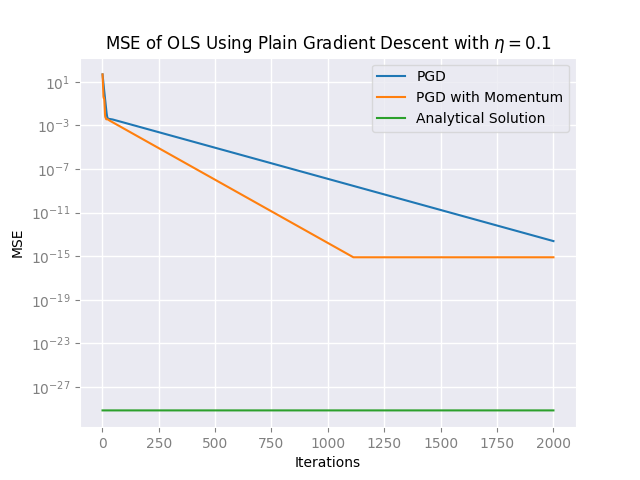
\includegraphics[width=\linewidth]{figures/all_plots/plain_mse_pr_iter_eta_1e-1.png}
    \caption{Plain gradient descent (PGD) with and without momentum compared to the analytical solution, with a constant learning rate of $\eta = 0.1$ and a momentum parameter $\gamma = 0.5$.}
    \label{fig:plainVSanalytical}
\end{figure}

Next, we looked at our stochastic methods, with and without momentum. In this case we tried a linearly decaying learning rate to see if we would have any major improvements over plain gradient descent. In this case, the linearly decaying learning rate used was:
\[
\eta_t = (1- \frac{t}{5})0.1 + \frac{t}{5} 0.001
\]
where we found the value $\eta_0 = 0.1$ after a few tests, as well as consulting the literature. We also kept the mini-batch size fixed at 4, which we found produced decent values in this case. The comparison of the MSE with and without momentum as a function of epochs is displayed in figure \ref{fig:sgdVSanalytical}. 
\begin{figure}
    \centering
    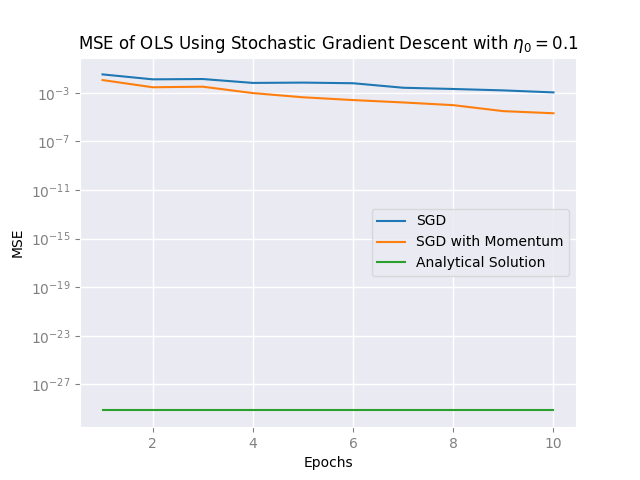
\includegraphics[width=\linewidth]{figures/all_plots/sgd_mse_pr_epoch_eta_1e-1.png}
    \caption{Stochastic gradient descent (SGD) with and without momentum compared to the analytical solution, with a constant learning rate of $\eta_0 = 0.1$ and a momentum parameter $\gamma = 0.5$. The size of the mini-batches is also fixed at 4.}
    \label{fig:sgdVSanalytical}
\end{figure}

We timed our methods, and as expected, stochastic gradient descent gave us results quicker, with minimal detriment to the MSE. \textcolor{red}{(We should time our results with plain and SGD and mention here that SGD is quicker.)} From this point on, we will therefore continue using stochastic instead of plain gradient descent for computational efficiency.

Next, we looked at the methods with adaptive learning rates. All methods were initialized with the same global learning rate $\eta = 0.1$ to begin with, as this was the best result in both of our previous tests. We wanted to see how the different methods adapted the learning rate over time, and if this behavior was consistent with the theory. The learning rates as a function of epochs can be seen in figure \ref{fig:learningratesGD}, and the development of the MSE over epochs in figure \ref{fig:MSEGD}. We expect smoother graphs with faster convergence in methods with momentum, \textcolor{red}{true/false}.
\begin{figure}
    \centering
    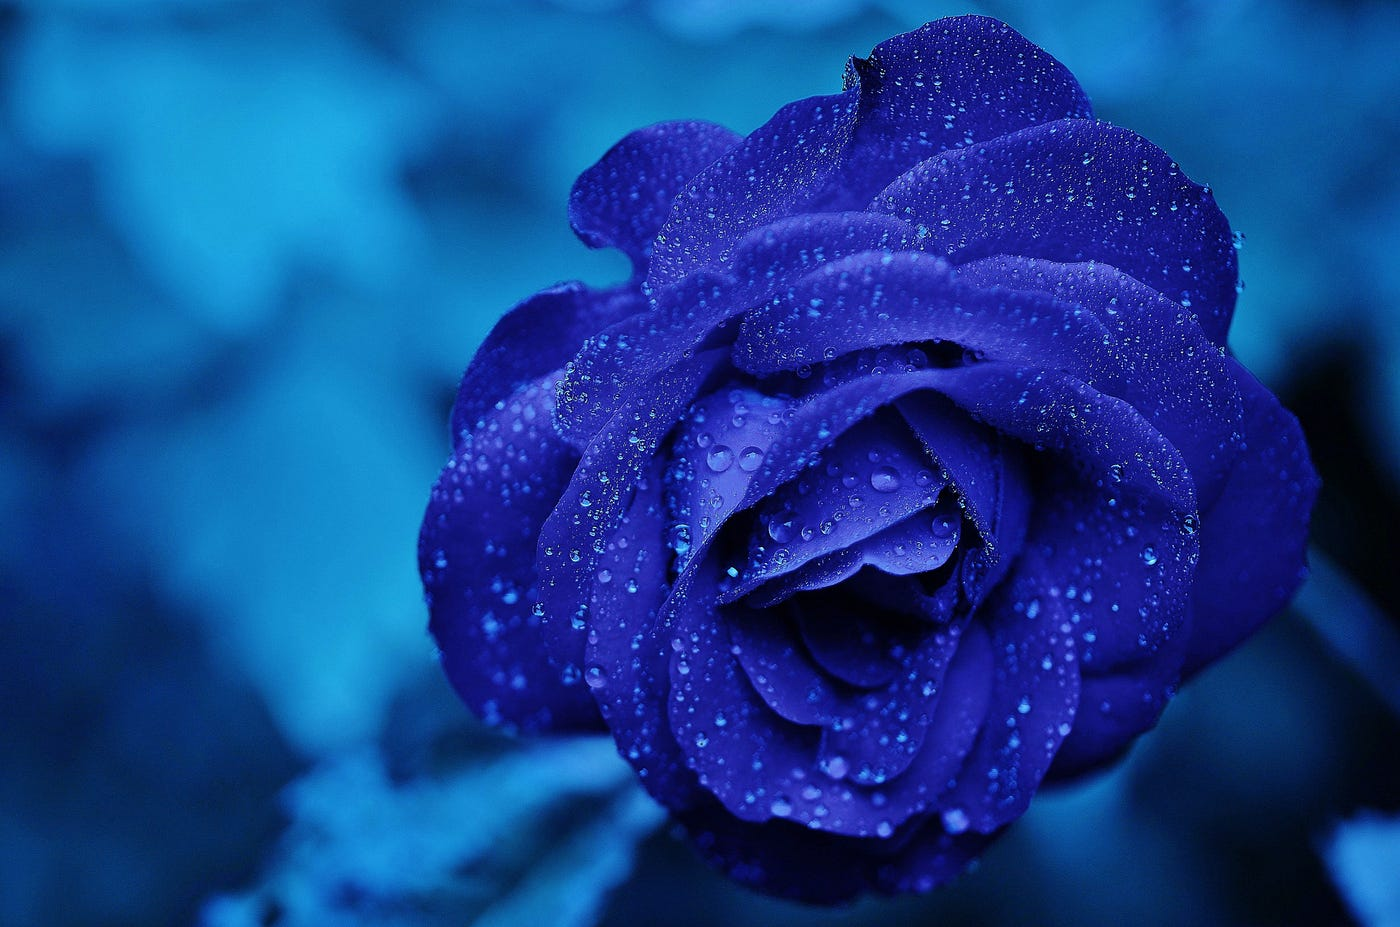
\includegraphics[width=0.5\linewidth]{figures/placeholders/learningratesGD.png}
    \caption{\textcolor{purple}{Plot of 3 subplots showing SGD w and w/o momentum for each of the three methods of adaptable learning rates.  Function of number of epochs. Learning rate on y-axis. See photo on Emma's phone.}}
    \label{fig:learningratesGD}
\end{figure}

\begin{figure}
    \centering
    
\includegraphics[width=0.5\linewidth]{figures/placeholders/MSEGD.png}
    \caption{\textcolor{purple}{Plot of 3 subplots showing SGD w and w/o momentum for each of the three methods of adaptable learning rates.  Function of number of epochs. MSE on y-axis.}}
    \label{fig:MSEGD}
\end{figure}

As part of our testing process, we compared the performance of our gradients to that of the automatic differentiation library Autograd \cite{autograd}. Since our tests pass\footnote{Tests can be found on our GitHub: \url{https://github.com/emmastorberg/FYS-STK4155_Project2/blob/main/tests.py}}, we expected our implementations to give quite similar results as these pre-existing methods, which they did. 

Up to this point, we have only looked at OLS. When we use ridge regression instead, there is the additional hyperparameter $\lambda$ to consider. We performed a grid search to determine what combination of $\lambda$ and gradient descent method to choose, and tested $\lambda \in \text{\textcolor{red}{(value)}}$ against each of the seven methods we tested for OLS in figures \ref{fig:learningratesGD} and \ref{fig:MSEGD}. The grid search table can be seen in figure \ref{fig:gridsearch_ridge}, where we can visually determine the best method as \textcolor{red}{(add method here)}, with $\lambda = \text{\textcolor{red}{(value)}}$. \textcolor{red}{An additional table showing the results of a grid search for finding the best $R^2$ score can be found in appendix (LETTER). (Remove if we don't do this.)} 
\begin{figure}
    \centering
    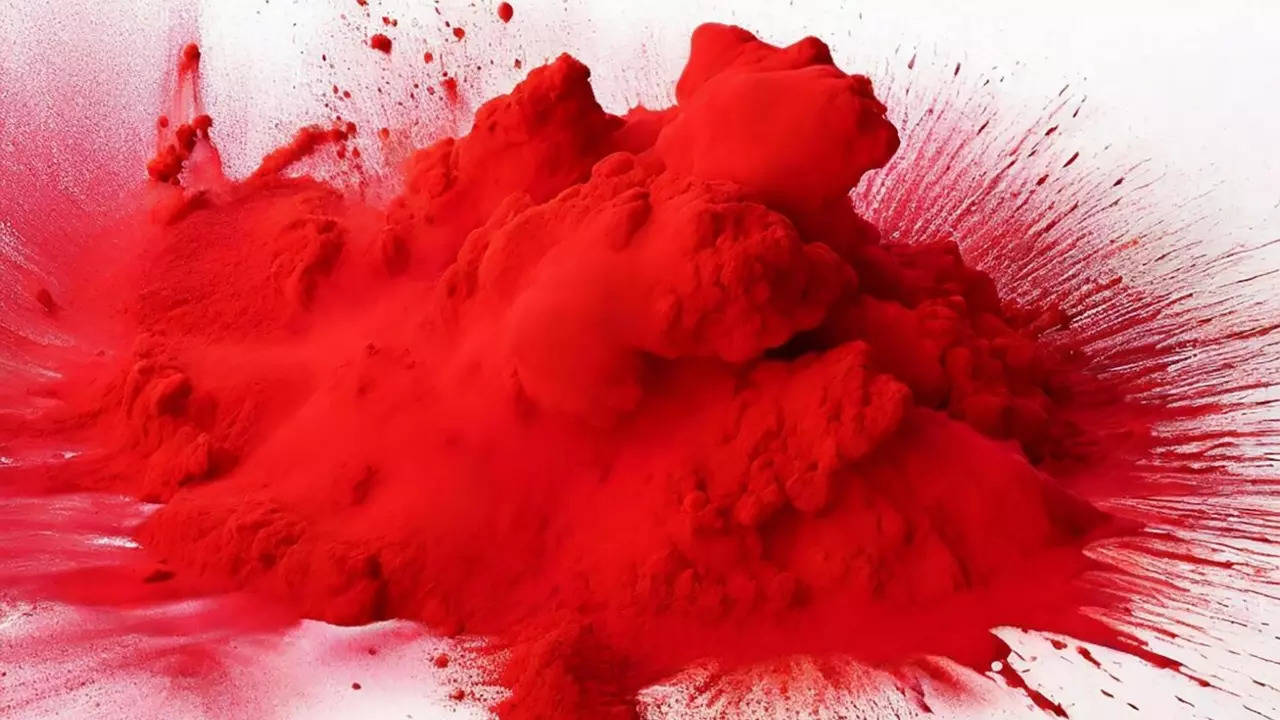
\includegraphics[width=0.5\linewidth]{figures/placeholders/gridsearch_ridge.png}
    \caption{\textcolor{purple}{Grid search table of the seven possible methods compared for different values of the hyperparameter $\lambda$}}
    \label{fig:gridsearch_ridge}
\end{figure}

\subsection{Numerical Prediction with Neural Network}
We saw that the optimal gradient descent methods for linear regression were \textcolor{red}{(method)} and \textcolor{red}{(method)}, with $\lambda = \text{\textcolor{red}{(value)}}$ for ridge regression. There is an enormous number of possible neural networks we can create even with only the relatively few gradient descent methods and activation functions at our disposal, in addition to the limitation of computation time. We eliminated a few degrees of freedom here by sticking to \textcolor{red}{(method)} as our gradient descent method (based on its performance in the experiments up to this point), and with ReLU as the activation function for the outer layer, guided by the theoretical intuition of what values it can produce (only positive values; the range of our polynomial $f(x) = \text{\textcolor{red}{(polynomial)}}$ is positive real numbers only).

To construct the network, we tried to sequentially eliminate degrees of freedom by fixating certain parameters, and thereafter exploring slight modifications to these. We started by using the same number of nodes per layer, and performing a grid search to find the best combination. The results of this are shown in figure \ref{fig:gridsearch_numpred_layers_nodes}, with sigmoid activating all hidden layers, and ReLU on the output layer.
\begin{figure}
    \centering
    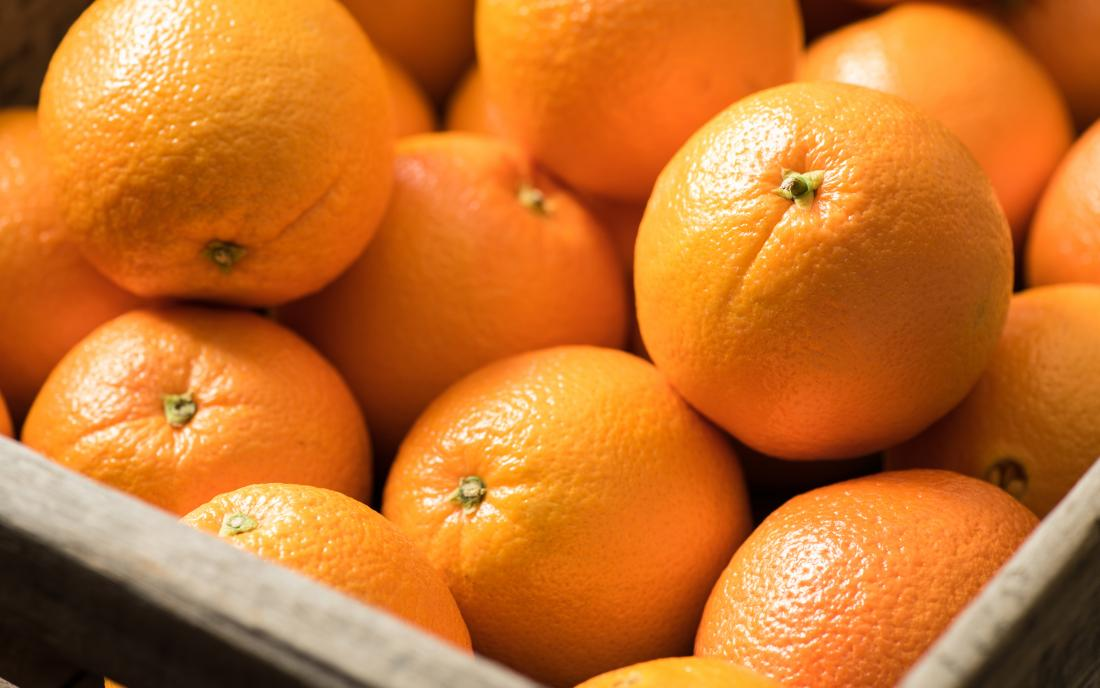
\includegraphics[width=0.5\linewidth]{figures/placeholders/gridsearch_numpred_layers_nodes.png}
    \caption{\textcolor{purple}{Heat map showing the MSE for the numerical NN predictions, as a function of hidden layers (1-5) and nodes in each hidden layer (1-10)}}
    \label{fig:gridsearch_numpred_layers_nodes}
\end{figure}

As we can see, a network with \textcolor{red}{(nodes and layers)} works the best out of the options we tested. Next, we tried varying what activation functions to use on the hidden layers. The plot of the resulting MSEs is shown in figure \ref{fig:activationfunctions_cost_numpred}. It seems clear that \textcolor{red}{(activation function)} activating the hidden layers is best in this case, so a neural network with \textcolor{red}{(NN explained here)} became the basis for further modifications in hopes of improving performance. 
\begin{figure}
    \centering
    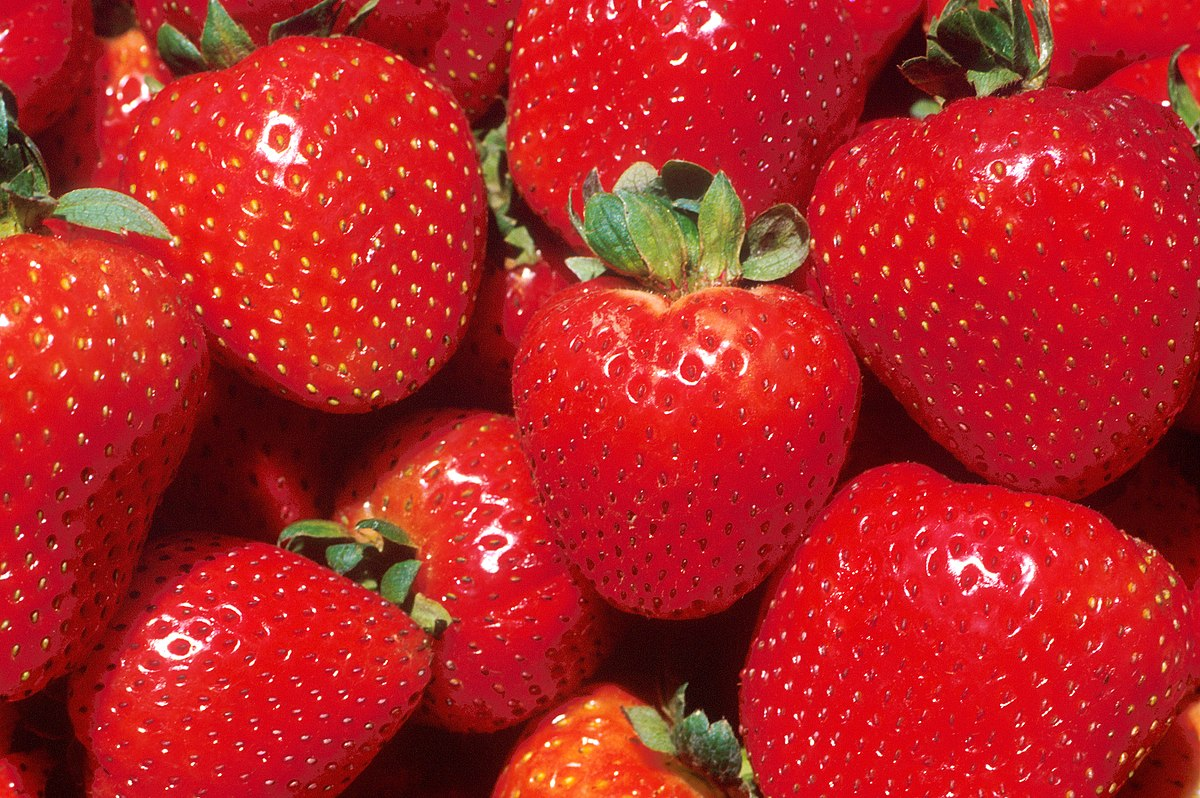
\includegraphics[width=0.5\linewidth]{figures/placeholders/activationfunctions_cost_numpred.png}
    \caption{\textcolor{purple}{Cost as a function of number of epochs, testing for four different neural networks. They all have the size determined in the grid search, but now we want to see if changing the activation of the hidden layers gives us any improvements.}}
    \label{fig:activationfunctions_cost_numpred}
\end{figure}

With slight variations to the hidden layers, the number of nodes in them and what activation functions to use at each stage, we arrived at our best-performing network for this task. The hyperparameters used to create it can be seen in table \ref{tab:numericalprediction}: 
\begin{table}[h!]
  \centering
  \small
  \begin{tabular}{|c|c|}
    \hline
    \textbf{Hyperparameter} & \textbf{Value} \\
    \hline
    Number of data points & $n = $ \\
    \hline
    Scaling of data & \texttt{StandardScaler} \\
    \hline
    Number of mini-batches (epochs) & $M =$ \\
    \hline
    Mini-batch size & $\frac{n}{M} = $ \\
    \hline
    Gradient descent method & Adam \\
    \hline
    Initial learning rate & $\eta = $ \\
    \hline
    Decay rate of first moment & $\rho_1 =$ \\
    \hline
    Decay rate of second moment & $\rho_2 = $ \\
    \hline
    Numerical stability constant & $\delta = $ \\
    \hline
    Cost function & MSE \\
    \hline
    Input layer & Size, activation \\
    \hline
    Layer 2 & Size, activation \\
    \hline
    Layer 3 & Size, activation \\
    \hline
    Output layer & Size, activation \\
    \hline
  \end{tabular}
  \caption{The chosen hyperparameters for best performance in numerical prediction task.}
  \label{tab:numericalprediction}
\end{table}

The neural network described \textcolor{blue}{above} was able to predict with an accuracy of \textcolor{red}{(value)}\%. The MSE of our best-performing neural network, OLS and ridge regression compared to a neural network created with Scikit-Learn can be seen in figure \ref{fig:numericalprediction}; a similar comparison of $R^2$ score can be found in figure \ref{fig:numericalpredictionR2} in appendix \textcolor{red}{(LETTER)}. We also show the predictions made by each method in figure \ref{fig:predictioncomparison}.

\begin{figure}
    \centering
    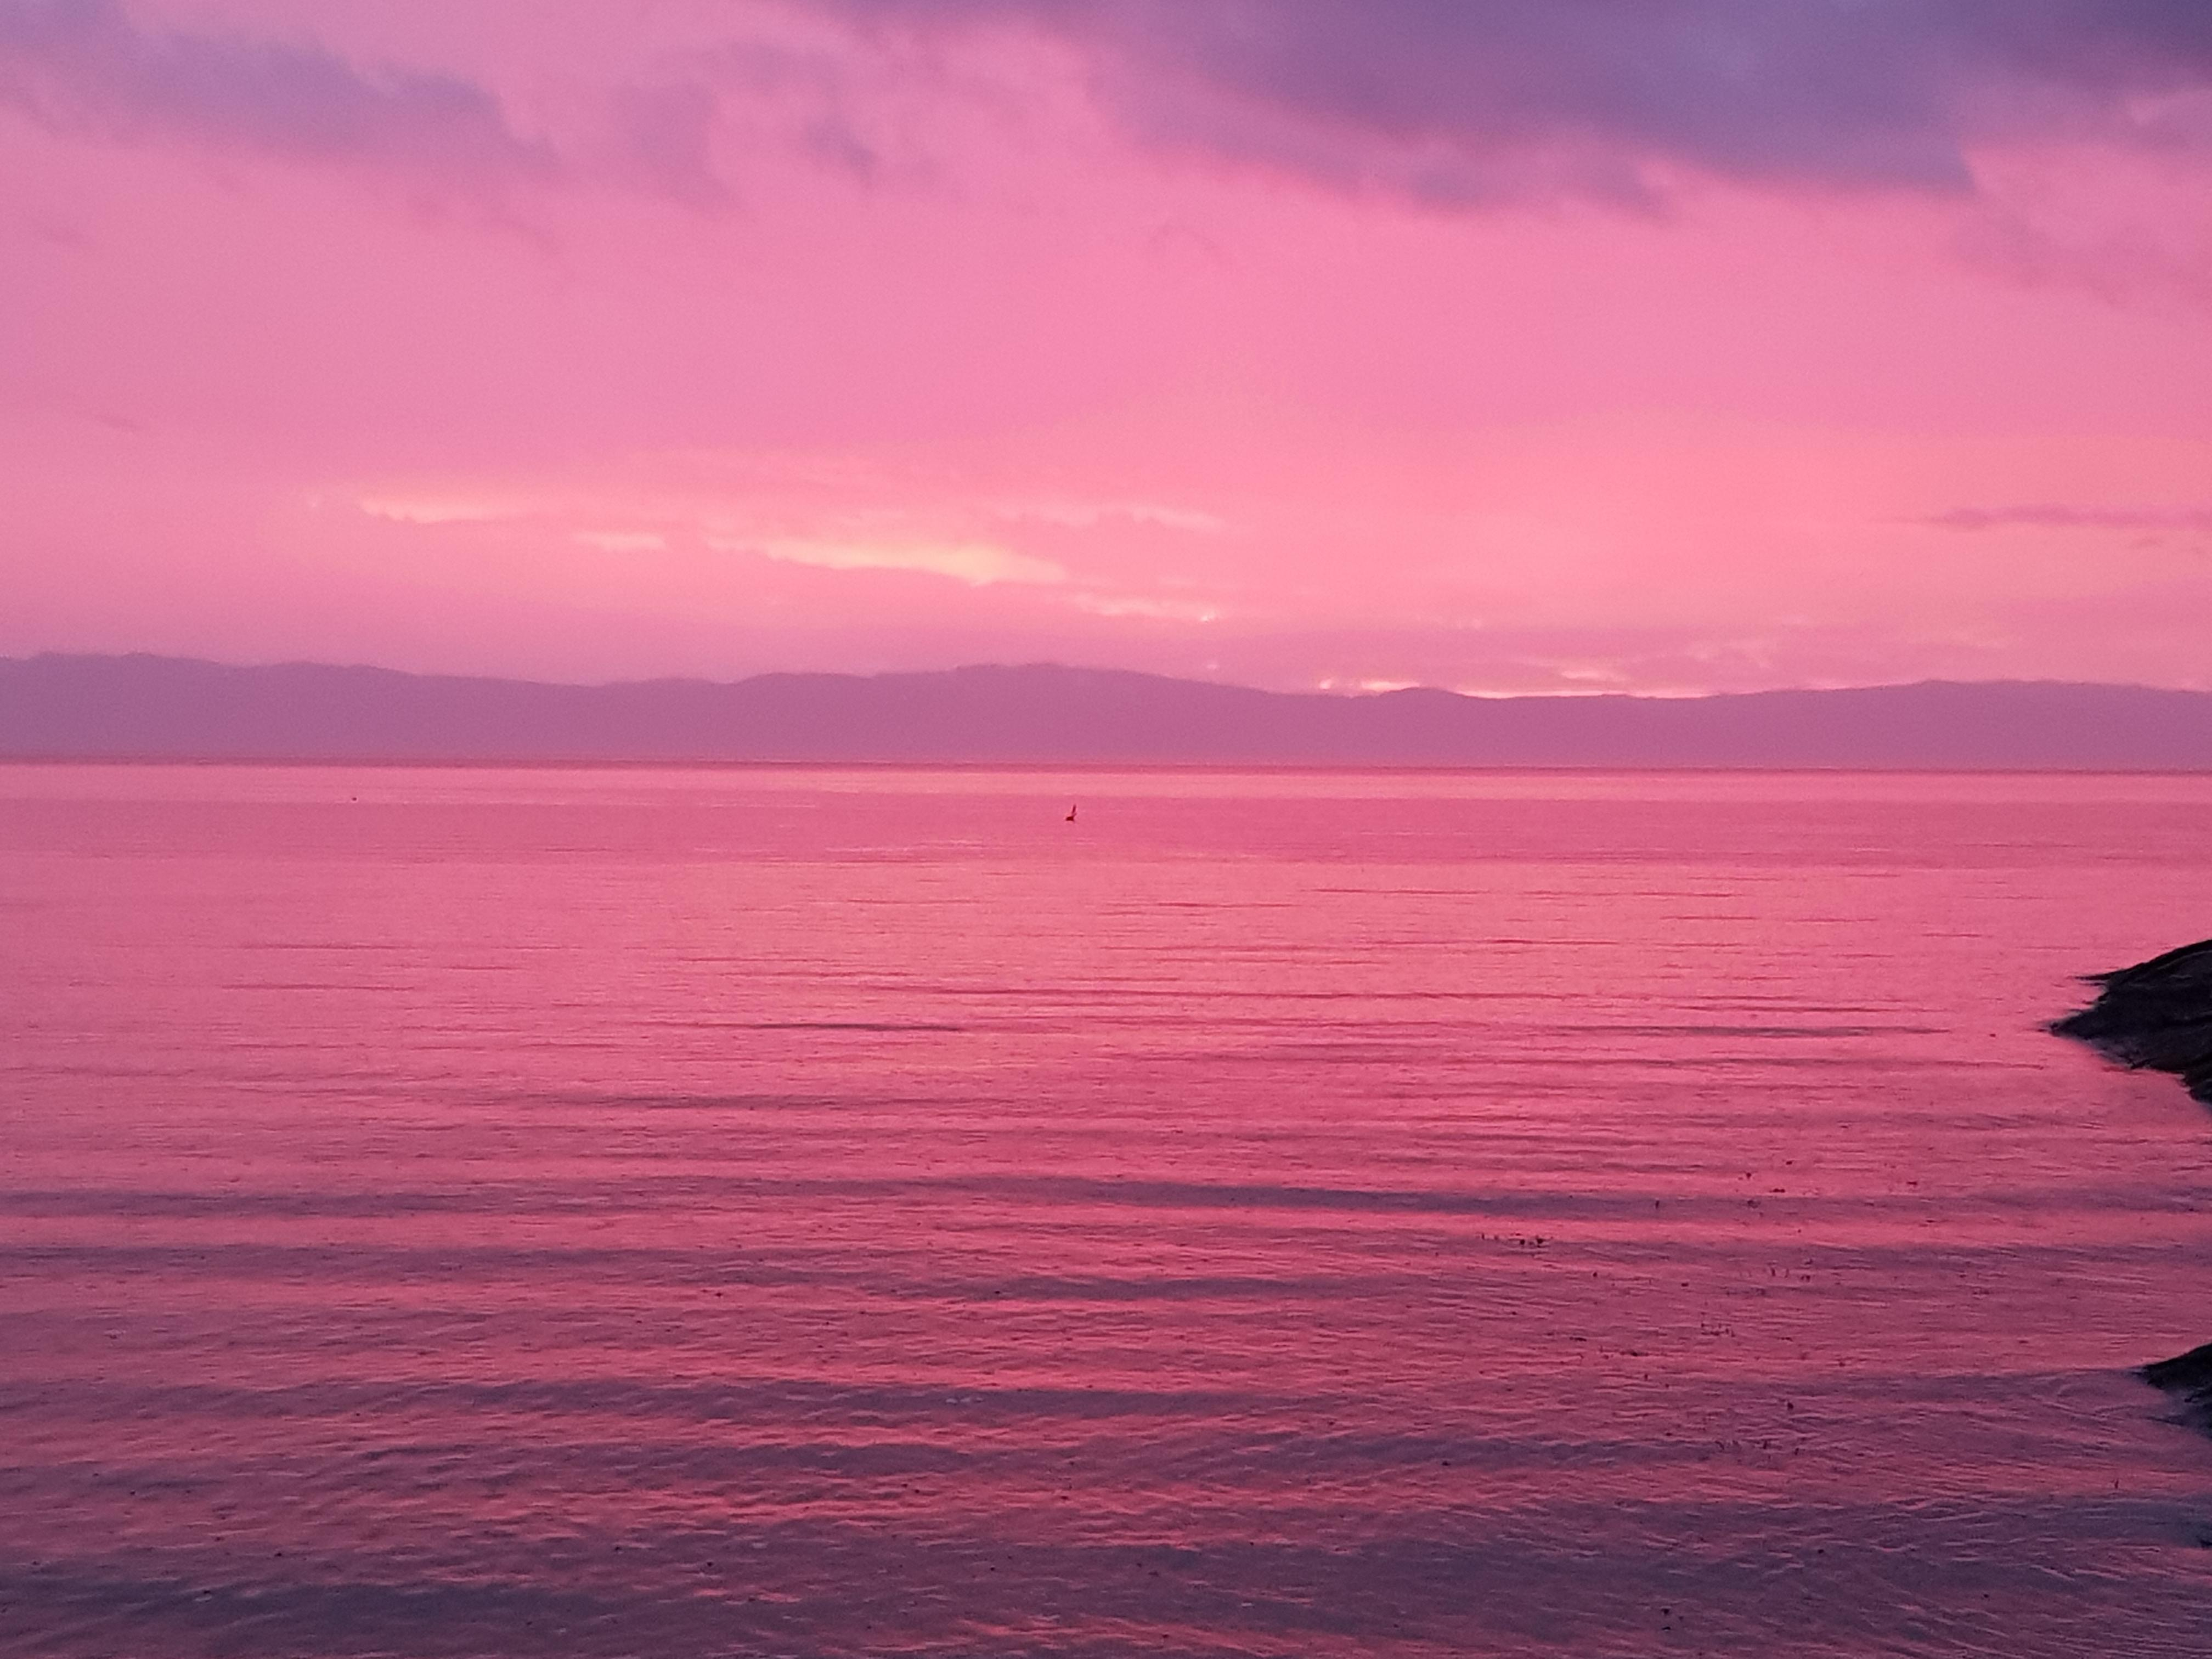
\includegraphics[width=0.5\linewidth]{figures/placeholders/numericalprediction.png}
    \caption{\textcolor{purple}{MSE as a function of epochs for OLS, Ridge and neural network (optimal version of all three methods). We also need a sklearn comparison here.}}
    \label{fig:numericalprediction}
\end{figure}

\begin{figure}
    \centering
    
\includegraphics[width=0.5\linewidth]{figures/placeholders/predictioncomparison.png}
    \caption{Comparison of predictions with optimal versions of all methods shown.}
    \label{fig:predictioncomparison}
\end{figure}

As we can see, it seems that the best method overall for this task is \textcolor{red}{(method)} with parameters \textcolor{red}{(parameters)}. 

\subsection{Classification with Neural Network}
Moving on to the classification task, we once again faced the issue of an extreme number of possibilities to test in order to construct the best-performing network. We limited our scope to only \textcolor{red}{(method)} with parameters \textcolor{red}{(parameters)}.

\subsubsection{First Attempt with Our Own Implementation}
Similar to the procedure in the creation of a network for numerical prediction, to make the optimal network for binary classification, we first employed a grid search of a fixed number of nodes per layer, and thereafter we altered the activation function on the hidden layers to see what gave the best results. In this process, we uncovered an error in the implementation. It looked as though the network predicted the average of the target vector, which gave an accuracy approximately equal to the frequency of target value 1 since we are working with binary classification. 

The source of the error, as well as its solution, remains elusive. We studied the implementation and behavior of our network extensively. Unit testing also passes for all of our methods\footnote{See our GitHub: \url{https://github.com/emmastorberg/FYS-STK4155_Project2}}.  

We initially scaled our data with \texttt{StandardScaler}, which we thought might be the issue, but changing the scaling to \texttt{MinMaxScaler} (also from Scikit-Learn \cite{sklearnScaling}) offered only an incremental change (from an accuracy of approximately 0.62 to 0.63). All gradient descent methods had also passed rigorous unit testing, and we also knew from the experiments in the previous section on the numerical prediction task that our neural network code was capable of producing reasonable results from a theoretical standpoint. 

We tested our network on different datasets, including the iris dataset \cite{irisdataset}, which is a common and beginner-friendly dataset used for testing classification networks. Our implementation performs well on this dataset when scaled with \texttt{StandardScaler}, though not with \texttt{MinMaxScaler}. This showed that it was able to do some classification tasks, so we hoped the implementation was not the problem, but rather that the choice of parameters happened to lead us to a local minimum, which is why the accuracy stopped improving at an early iteration. However, an identical instantiation with PyTorch, an optimized tensor library for deep learning \cite{pytorch}, creates a network that is able to classify the data points without issue, so the instantiation and choice of parameters is most likely not the problem.

These confusing findings left us with an unclear path towards analyzing our code implementation on breast cancer data, as was the goal of this project. We found that through trial and error, we could achieve accuracy as high as \textcolor{red}{(accuracy)} \%. However, seeing as this is a multiclass rather than binary classification problem, continuing to work with this network and dataset will leave us unable to compare our results to a logistic regression, nor will we be exploring the application of machine learning methods in the medical field, as was our initial motivation.

Therefore we ultimately made the decision to continue working with the breast cancer data using PyTorch to explore the optimal instantiation of a network for such a dataset. The resulting neural network will also be compared to a logistic regression. 

\subsubsection{Continued Exploration with PyTorch}
Our search for the optimal set of hyperparameters for the task was in part systematic, and in part educated guesswork and trial and error. The first systematic test was a grid search, where we fixed the number of nodes in each layer. Throughout this task, we always used sigmoid as the activation function. A grid search table showing the best combination of number of layers and nodes per layer (with sigmoid activating all layers) is shown in figure \ref{fig:gridsearch_layers_nodes}. 

% our final activation function, and kept the activation functions of the hidden layers the same. Of our four options, having \textcolor{red}{(activation function)} activate all hidden layers resulted in highest accuracy overall. 

\begin{figure}
    \centering
    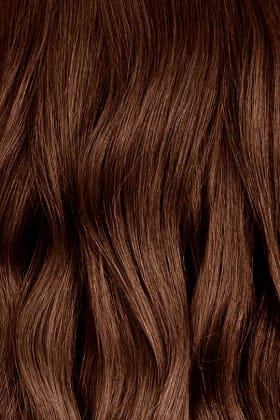
\includegraphics[width=0.5\linewidth]{figures/placeholders/gridsearch_layers_nodes.png}
    \caption{\textcolor{purple}{Heat map showing the accuracy for the neural net (on the cancer dataset), as a function of hidden layers (1-5) and nodes in each hidden layer (1-10)}}
    \label{fig:gridsearch_layers_nodes}
\end{figure}

As we can see, the optimal result seems to be \textcolor{red}{(nodes in each layer explained here)}. Using this as a starting point for further exploration, we continued looking into if a different set of activation functions for the hidden layers would have any effect. In figure \ref{fig:activationfunctions_cost}, we see all four options for activation functions on a neural network with \textcolor{red}{(nodes in each layer explained here)}, as determined in figure \ref{fig:gridsearch_layers_nodes}. We see that \textcolor{red}{(activation function)} works \textcolor{red}{better/worse} than our initial test using sigmoid everywhere, so we continued tweaking a network in the form of \textcolor{red}{best finding here}.

\begin{figure}
    \centering
    
\includegraphics[width=0.5\linewidth]{figures/placeholders/activationfunctions_cost.png}
    \caption{\textcolor{purple}{Cost as a function of number of epochs, testing for four different neural networks. They all have the size determined in the grid search, but now we want to see if changing the activation of the hidden layers gives us any improvements.}}
    \label{fig:activationfunctions_cost}
\end{figure}

Through less organized trial and error testing, we began with the optimal network so far, with size \textcolor{red}{(layer and node info)} and \textcolor{red}{(activation function)} on all hidden layers. We were able to find that with \textcolor{red}{(activation function on hidden layers)} and \textcolor{red}{(alternative neural network structure)}, we could now achieve an accuracy of up to \textcolor{red}{(accuracy)}\% for the Wisconsin Breast Cancer dataset. \textcolor{green}{We expected from the theory that ReLU would do well, and in particular, offer faster convergence than the other methods. This applies/does not apply in this case as well.} The full set of chosen hyperparameters for this neural network are shown in table \ref{tab:classificationtask}.

\begin{table}[h!]
  \centering
  \small
  \begin{tabular}{|c|c|}
    \hline
    \textbf{Hyperparameter} & \textbf{Value} \\
    \hline
    Number of data points & $n = $ \\
    \hline
    Scaling of data & \texttt{StandardScaler} \\
    \hline
    Number of mini-batches (epochs) & $M =$ \\
    \hline
    Mini-batch size & $\frac{n}{M} = $ \\
    \hline
    Gradient descent method & Adam \\
    \hline
    Initial learning rate & $\eta = $ \\
    \hline
    Decay rate of first moment & $\rho_1 =$ \\
    \hline
    Decay rate of second moment & $\rho_2 = $ \\
    \hline
    Numerical stability constant & $\delta = $ \\
    \hline
    Cost function & Cross-entropy \\
    \hline
    Input layer & Size, activation \\
    \hline
    Layer 2 & Size, activation \\
    \hline
    Layer 3 & Size, activation \\
    \hline
    Output layer & Size, activation \\
    \hline
  \end{tabular}
  \caption{Table showing hyperparameters chosen for best-performing neural network in classification task}
  \label{tab:classificationtask}
\end{table}
%\textcolor{magenta}{Figure: Activation functions. Plot the accuracy of the network (on cancer data) with different combinations of activation functions [leaky relu, relu, only sigmoid, softmax] (although I believe all should have sigmoid in the final layer), as a function of layers. (I think we should have a fixed number of nodes, unless we want to grid search this and choose the best)} \\ 
%\textcolor{purple}{Alternative figure to the one above. The same idea, but with the best layer and node size from the first heatmap/a grid search, as a function of epochs. This makes us able to visualize which activation function converges faster. I think this is a better plot} \\

%\textcolor{purple}{Figure: Accuracy for [SGD (with and without momentum), Adagrad (with and without momentum), RMSprop and Adam] (on the legend) as a function of epochs, with a fixed learning rate}
%We expect them to converge, some faster than others. With momentum should converge faster.

The network as described \textcolor{blue}{above} has \textcolor{red}{(accuracy)}\% accuracy in its predictions overall. However, we must also consider what type of inaccuracy is most prevalent before determining this is the best network for the task. False positive and negative rate can be seen in the confusion matrix in figure \ref{fig:confusionmatrix}.
\begin{figure}
    \centering
    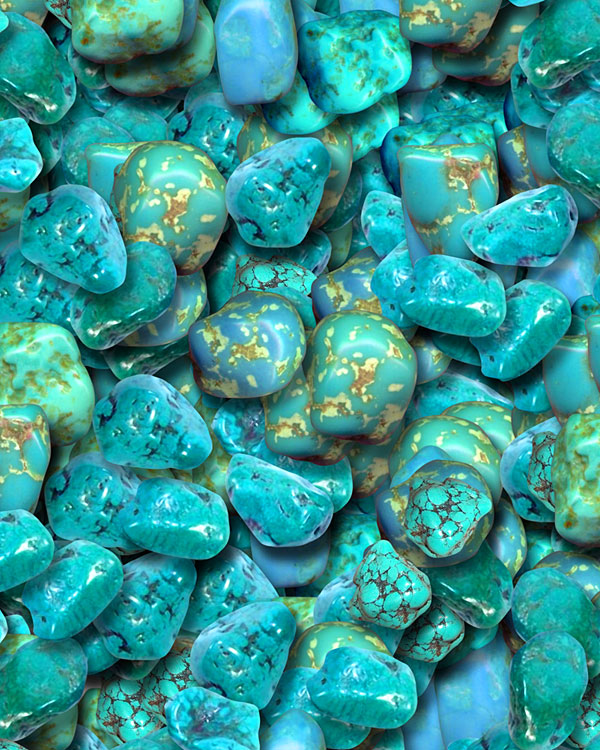
\includegraphics[width=\linewidth]{figures/placeholders/confusionmatrix.png}
    \caption{\textcolor{purple}{Confusion matrix for the neural net (on the cancer dataset, counting the number of TP, TN, FN and FP)}}
    \label{fig:confusionmatrix}
\end{figure}

% INCLUDE THIS PARAGRAPH IF ANOTHER PLOT IS NECESSARY; OTHERWISE, MOVE TO DISCUSSION.

% We tuned our model again to lower FN rate. The new confusion matrix can be shown in figure \ref{fig:confusionmatrix2}.
% \begin{figure}
%     \centering
%     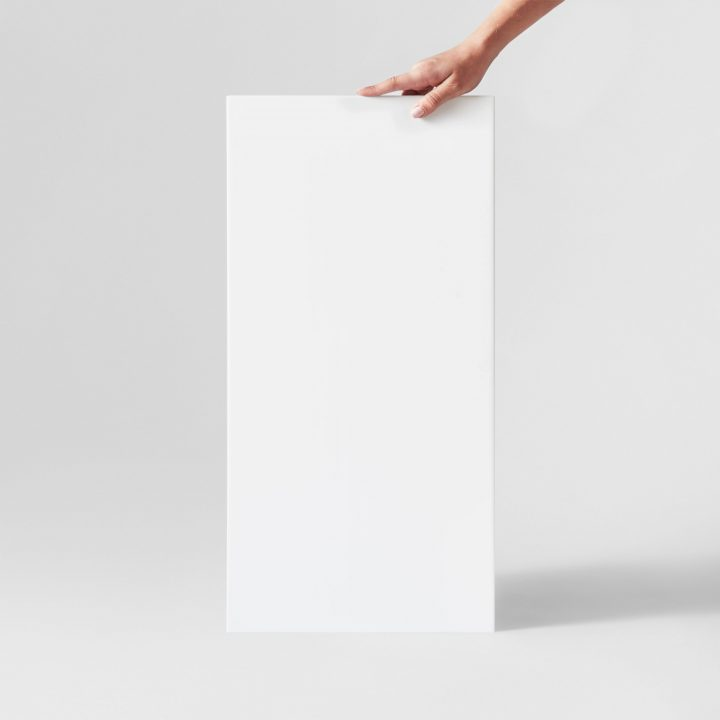
\includegraphics[width=0.5\linewidth]{figures/placeholders/confusionmatrix2.png}
%     \caption{\textcolor{purple}{Second confusion matrix for the neural net (on the cancer dataset, counting the number of TP, TN, FN and FP). Should definitely have less FN than FP this time around.}}
%     \label{fig:confusionmatrix2}
% \end{figure}

\subsection{Classification with Logistic Regression}
As discussed, an alternative to a neural network requiring far less tuning is logistic regression. This corresponds to a network with no hidden layers, activated by the sigmoid function. The resulting confusion matrix is shown in figure \ref{fig:logreg}. 
\begin{figure}
    \centering
    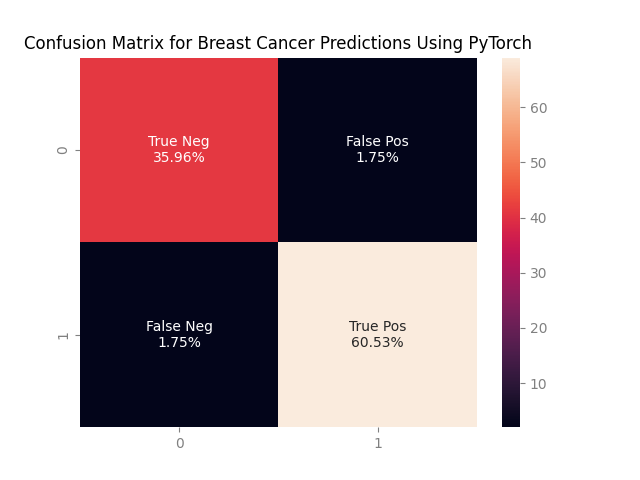
\includegraphics[width=\linewidth]{figures/plots/logreg.png}
    \caption{\textcolor{purple}{Confusion matrix from logistic regression}}
    \label{fig:logreg}
\end{figure}

As we can see, the performance of logistic regression alone is relatively poor compared to a neural network. However, we experienced first-hand that it requires much less time to set up and run, which should be taken into account when evaluating these methods.

\textcolor{magenta}{Should not be in report, but we should print accuracy/cf before and after scaling with the StandardScaler. Expect accuracy to increase. We can just cite on of our previous reports on scaling with StandardScaler}





\section{Discussion}
\textcolor{blue}{In general, did the results we saw align with the theory? Give a suggestion as to why/why not.}

In general, our results aligned quite with the theory, with a few hiccups in the classification part. In the first part of the project, the found that inclusion of 

First, we saw that our gradient descent methods were less accurate than using the analytical solutions. This makes sense, as they are numerical approximations. 

We also saw that dedicated linear regression methods worked better to predict values generated from a second-degree polynomial dataset than a neural network. This makes sense: Neural networks are universal approximators, and can be utilized for a range of tasks, but with some inaccuracy compared to methods capable of given exact solutions (such as OLS does in this case). 

\textcolor{blue}{What were the choices of hyperparameters, and what was the effect of choosing those specific ones?}

In the numerical prediction task, ...

\textcolor{blue}{Are neural networks worth all the tuning they require?}

Our goal is to minimize both false positives and false negatives. A false positive means unnecessary distress for the patient and their family, and wasted hospital resources on additional tests. A false negative, however, could be fatal if cancer goes untreated. Therefore, if the confusion matrix shows a high false negative rate, our loss function should be modified to penalize false negatives more heavily

\subsection{Limitation of methods}
Neural networks requires vast computational resources compared to regression methods. Wee see that the runtime increases significantly for our neural net compared to our logistic regression. \\

-  Our neural nets require tuning. \\

For linear data, like in the linear regression example
%\ref{sec:linear code}
a linear regression model is a better choice. 
\\
When predicting breast cancer, we often want practitioners to use the model as decision support, not as the single source of truth. This is less straightforward with our neural network compared to the logistic regression model from scikit-learn \textcolor{red} cite, where we examined feature importance. Although prediction and understanding are related, accurate predictions can still come from flawed models, making it difficult for practitioners to interact with the model.
\subsection{What we found}

\textcolor{purple}{We found that creating a neural network from scratch can lead to numerical instability. }

\textcolor{purple}{Using neural network on simple tasks that can be solved by regression methods is not worth the trouble of tuning.}

\textcolor{purple}{For future work, we will work on numerical stability. }

\section{Conclusion}
The project has given us a solid theoretical and practical introduction to the underlying methods that make neural networks function as they do. However, we also faced issues along the way with complicated implementations.

We aimed to create a neural network completely from scratch, including implementing the gradient descent methods that are used in the training process. Through experiments with each subsequent part that was implemented, we were able to produce a network that could predict numerical values based on data generated from a polynomial, initialized with \textcolor{red}{(parameters)}. Following these initial tests, we constructed a network that could predict breast cancer data. From a theoretical and empirical standpoint, this should be a task a neural network is well-suited to do, and with the PyTorch implementation we saw solid performance with a neural network with \textcolor{red}{(parameters)}.

Thus, we are left with an important question: Are neural networks always worth all the tuning they require? Based on our findings, the answer is clearly \emph{no}. Our first use-case, numerical prediction, showed that OLS (implemented with a variety of gradient descent methods) was better suited than our neural network to predict polynomial data. The classification task let us see both sides: While we experienced first-hand how numerical instability and the implementation of the complex algorithms involved in machine learning can lead to hidden errors, we also saw the power of neural networks when we implemented PyTorch and were able to predict breast cancer with \textcolor{red}{(accuracy)}\% accuracy. The neural network outperformed its counterpart logistic regression, at the expense of a degree of explainability and computational time. 

In summary, we achieved our goal of exploring the creation and different usages of neural networks, and despite issues with our implementation, we saw how they can be used to predict medical data, and in this way function as a diagnostic tool in the field of medicine. In the process, we gained understanding of the nuances in neural networks, such as the cases in which a neural network may not be the best choice. It is important to tailor the methods used to the specific situation, and weigh the advantages against the risks that are presented.

\clearpage

\onecolumn
\printbibliography[heading=bibnumbered, title=References]
\clearpage

\appendix
\section{Comparison of our Methods to Autograd}
\input{docs/autograd_comparison}
\clearpage

\section{Additional Plots}
\subsection{Plot Determining Fixed Learning Rate to Use}
\begin{figure}
    \centering
    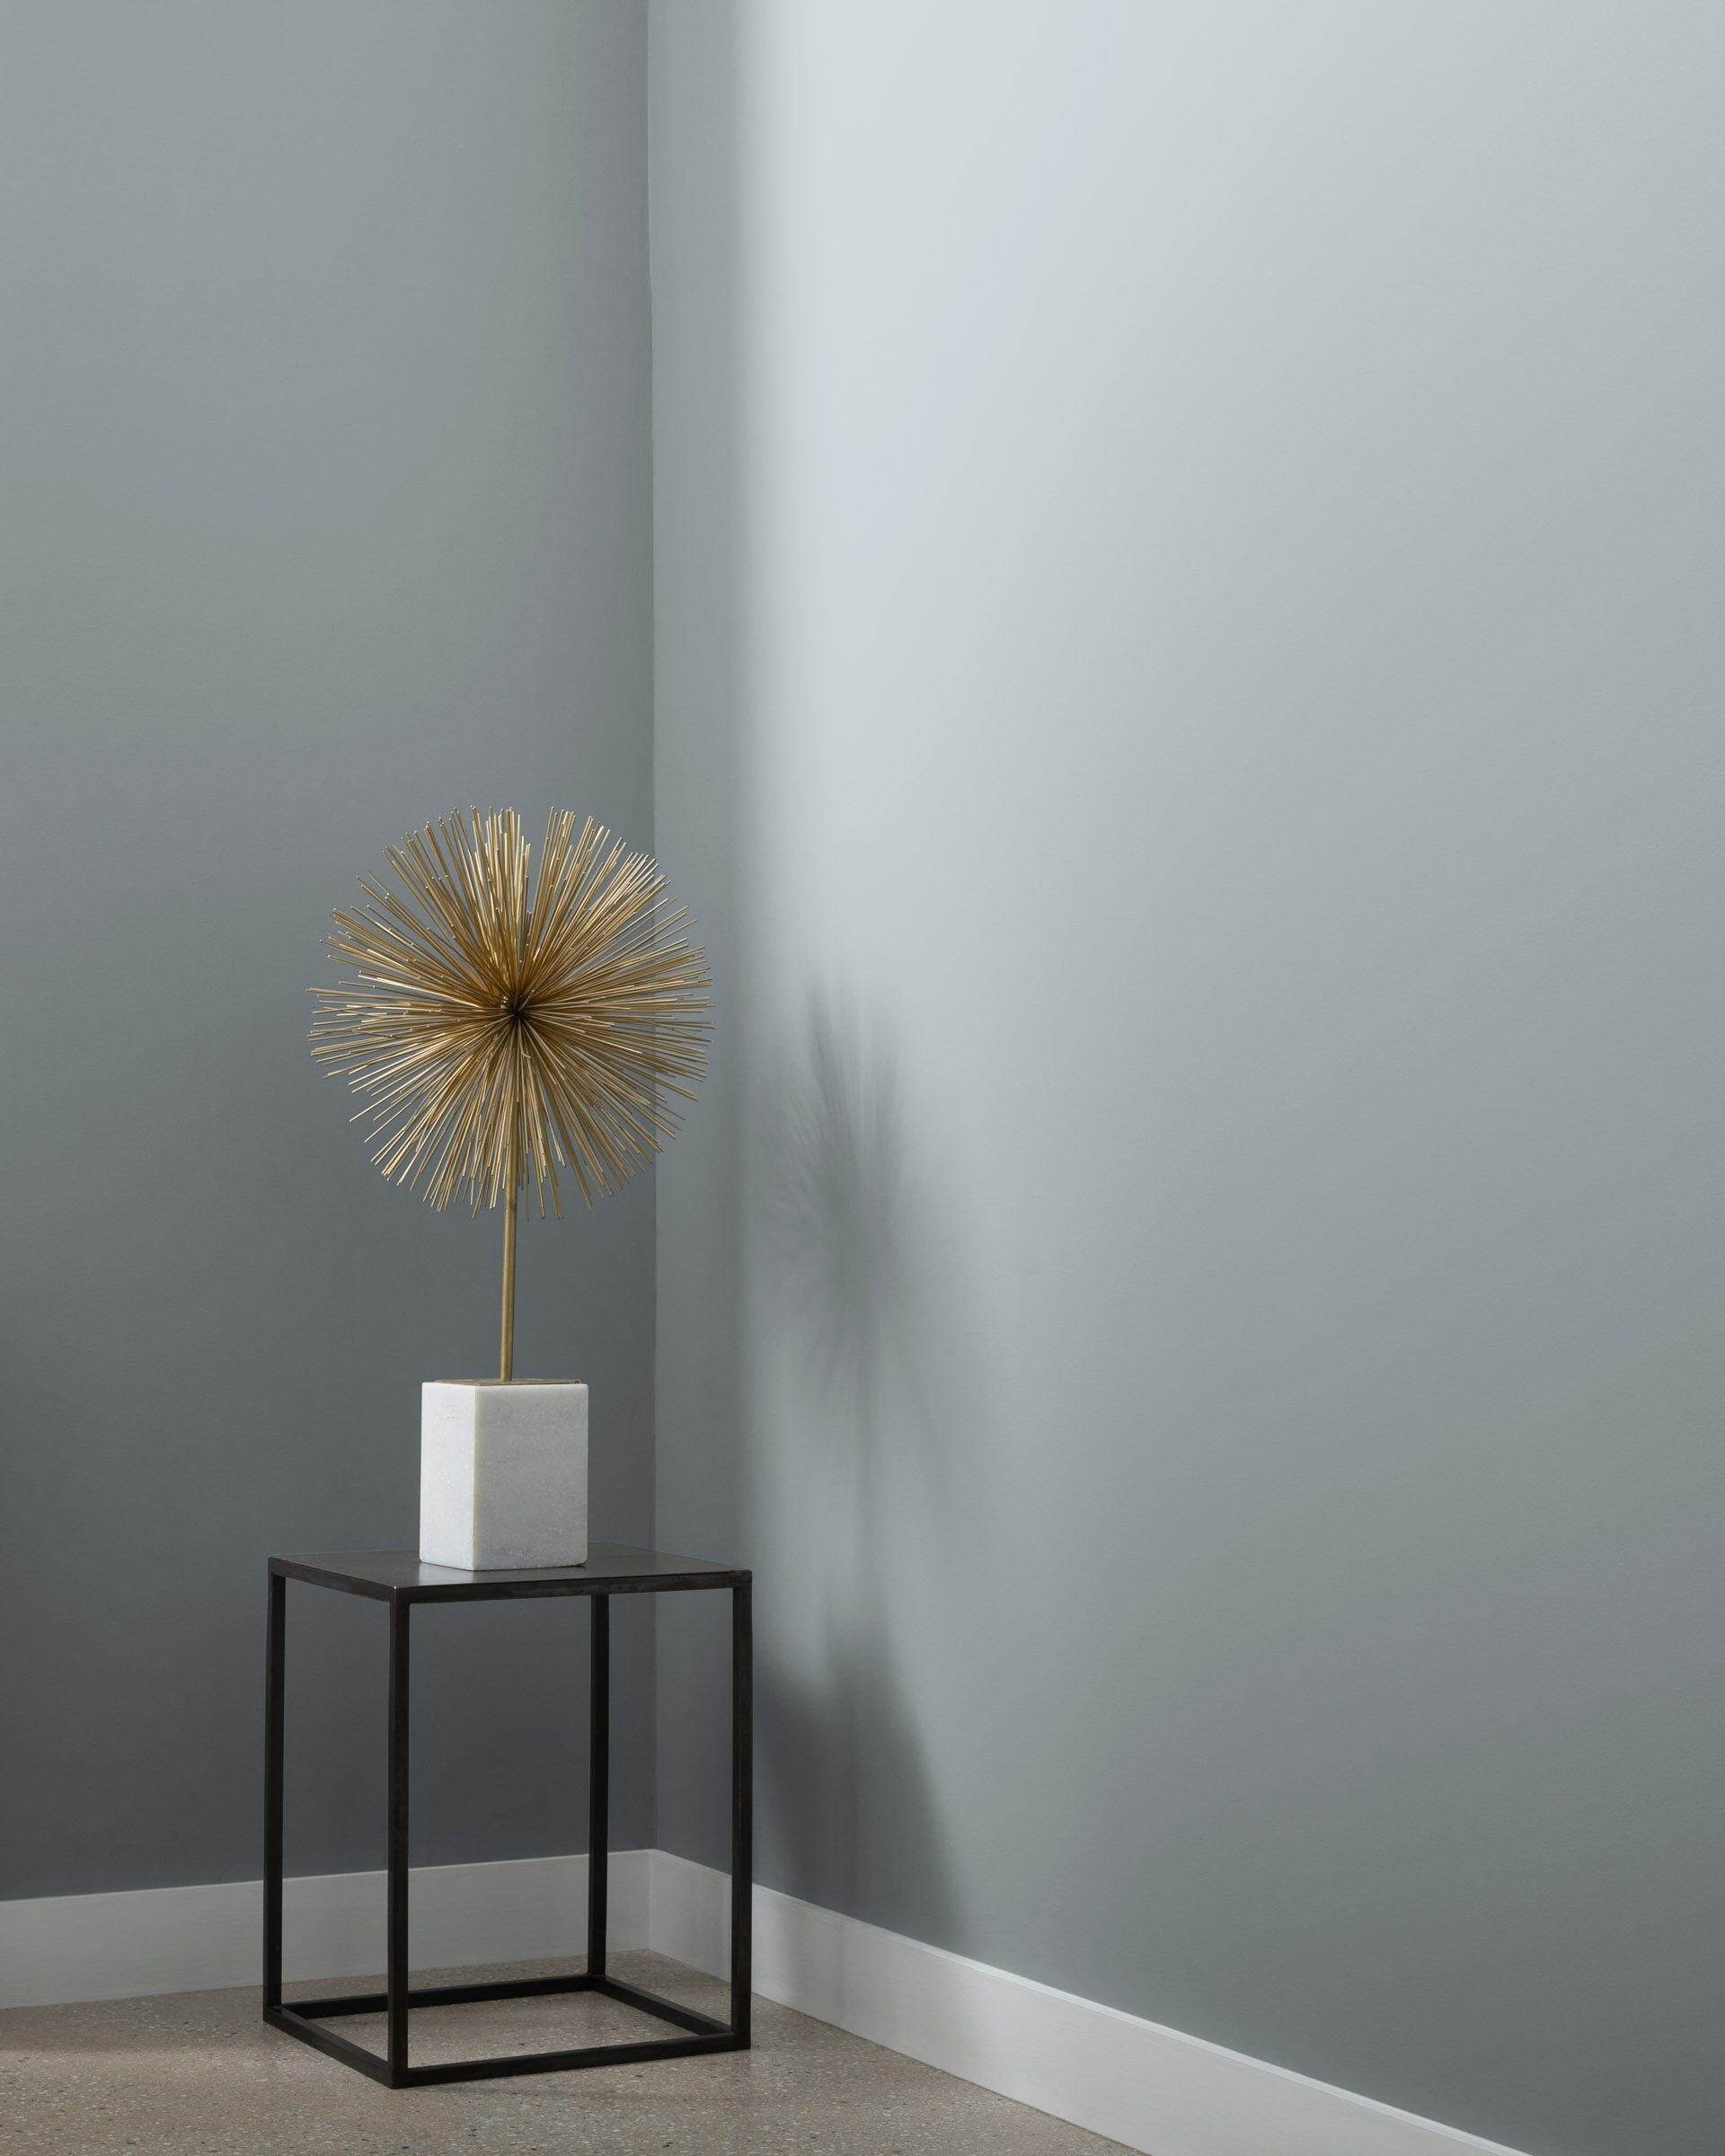
\includegraphics[width=0.5\linewidth]{figures/placeholders/plainWithDifferentLR.png}
    \caption{\textcolor{purple}{Plot showing our plain GD with 5 different learning rates as function of iterations.}}
    \label{fig:plainWithDifferentLR}
\end{figure}

\subsection{Grid Search Table Determining Best Hyperparameters for Ridge Regression with Respect to $R^2$ Score}
%Add figure code here if desired.

\subsection{$R^2$ Score of Experimentally-Determined Optimal Models}
\begin{figure}
    \centering
    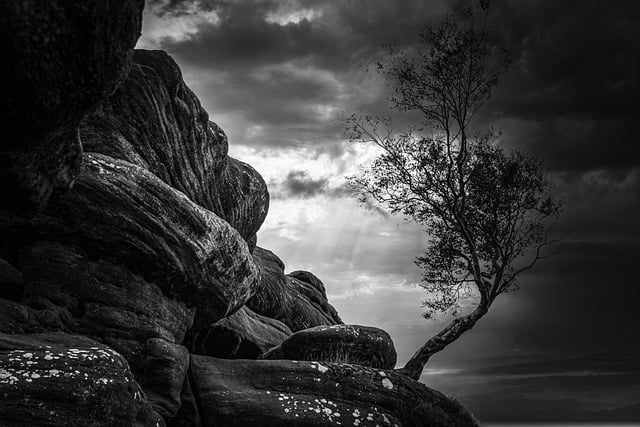
\includegraphics[width=0.5\linewidth]{figures/placeholders/numericalpredictionR2.png}
    \caption{\textcolor{purple}{$R^2$ score as a function of epochs for OLS, Ridge and neural network (optimal version of all three methods). We also need a sklearn comparison here.}}
    \label{fig:numericalpredictionR2}
\end{figure}
\clearpage

% COMMENT IN ADDITIONAL APPENDICES WHEN NECESSARY
% \section{\textcolor{red}{Appendix title TBA here}}
% \input{appendix}
% \clearpage

% \section{\textcolor{red}{Appendix title TBA here}}
% \input{appendix}
% \clearpage

\end{document}
